% THIS IS SIGPROC-SP.TEX - VERSION 3.1
% WORKS WITH V3.2SP OF ACM_PROC_ARTICLE-SP.CLS
% APRIL 2009
%
% It is an example file showing how to use the 'acm_proc_article-sp.cls' V3.2SP
% LaTeX2e document class file for Conference Proceedings submissions.
% ----------------------------------------------------------------------------------------------------------------
% This .tex file (and associated .cls V3.2SP) *DOES NOT* produce:
%       1) The Permission Statement
%       2) The Conference (location) Info information
%       3) The Copyright Line with ACM data
%       4) Page numbering
% ---------------------------------------------------------------------------------------------------------------
% It is an example which *does* use the .bib file (from which the .bbl file
% is produced).
% REMEMBER HOWEVER: After having produced the .bbl file,
% and prior to final submission,
% you need to 'insert'  your .bbl file into your source .tex file so as to provide
% ONE 'self-contained' source file.
%
% Questions regarding SIGS should be sent to
% Adrienne Griscti ---> griscti@acm.org
%
% Questions/suggestions regarding the guidelines, .tex and .cls files, etc. to
% Gerald Murray ---> murray@hq.acm.org
%
% For tracking purposes - this is V3.1SP - APRIL 2009

\documentclass{acm_proc_article-sp}
\usepackage{url}
\usepackage{amsmath}
\newcommand{\la}{\ensuremath{ \mathcal{L}}}
%\newcommand{\PL}{\ensuremath{ \mathcal{P}_{\alpha}}}
\newcommand{\PLB}{\ensuremath{ \mathcal{P}_{\alpha}}}
\newcommand{\PLC}{\ensuremath{ \mathcal{P}'_{\alpha}}}
\newcommand{\Sparse}{\ensuremath{ \mathcal{S}_{c,n}}}
\newtheorem{definition}{Definition}
\newtheorem{theorem}{Theorem}
\newtheorem{proposition}{Proposition}
\newtheorem{lemma}{Lemma}
\newtheorem{conjecture}{Conjecture}
\usepackage{subfig}
\usepackage{graphicx}

\begin{document}

\title{Peer-to-Peer storage of power-law graphs}
%
% You need the command \numberofauthors to handle the 'placement
% and alignment' of the authors beneath the title.
%
% For aesthetic reasons, we recommend 'three authors at a time'
% i.e. three 'name/affiliation blocks' be placed beneath the title.
%
% NOTE: You are NOT restricted in how many 'rows' of
% "name/affiliations" may appear. We just ask that you restrict
% the number of 'columns' to three.
%
% Because of the available 'opening page real-estate'
% we ask you to refrain from putting more than six authors
% (two rows with three columns) beneath the article title.
% More than six makes the first-page appear very cluttered indeed.
%
% Use the \alignauthor commands to handle the names
% and affiliations for an 'aesthetic maximum' of six authors.
% Add names, affiliations, addresses for
% the seventh etc. author(s) as the argument for the
% \additionalauthors command.
% These 'additional authors' will be output/set for you
% without further effort on your part as the last section in
% the body of your article BEFORE References or any Appendices.

\numberofauthors{1} %  in this sample file, there are a *total*
% of EIGHT authors. SIX appear on the 'first-page' (for formatting
% reasons) and the remaining two appear in the \additionalauthors section.
%

\author{Casper Petersen, Noy Rotbart,\\ Jakob Grue Simonsen and Christian Wulff-Nilsen \\ \\
\small{Department of Computer Science, University of Copenhagen} \\
\small{Universitetsparken 5, 2100 Copenhagen}\\
 \small{\texttt{\{cazz,noyro,simonsen,koolooz\}@diku.dk}} \\
 \small{phone: (+45) 29611674}
 }
 

\date{28 September 2015}
\maketitle
\begin{abstract}
The study of web graph compression assumes a centralised data structure which is undesired in peer-to-peer networks.
We propose an investigation on web graph dissemination using a theoretically appropriate method, adjacency labeling scheme. These are  methods that assigns labels to the vertices of a graph such that adjacency between them 
can be inferred directly from the assigned labels, without using a  centralized data structure.
We first provide a lower bound for the family of power-law graphs.  This  family has been used to model many types of networks, e.g. the Internet AS-level graph. Furthermore, we  provide an almost matching  upper bound for this family.
%We also provide an asymptotically near-optimal  labeling scheme for sparse graphs.
This upper bound is attained by pre-determining a threshold separating nodes of large degree and small degree that attempts to balance the storage required among the vertices. We then  validate the efficiency of our separation by  an experimental evaluation  using both synthetic data and real-world networks of up to hundreds of thousands of vertices. 
\end{abstract}

% A category with the (minimum) three required fields
\category{H.4}{Information Systems Applications}{Miscellaneous}
%A category including the fourth, optional field follows...
\category{D.2.8}{Software Engineering}{Metrics}[complexity measures, performance measures]

\terms{Theory}

\keywords{ACM proceedings, \LaTeX, text tagging} % NOT required for Proceedings
% !TEX root = WWW.tex


\section{Introduction}
A body of work on large, real-world networks  deals with the difficulties of storing them and to effectively resolve queries on them; examples of techniques are
compression~\cite{boldi2004webgraph,boldi2011layered} and dissemination  the underlying graphs of these networks over several machines~\cite{gonzalez2012powergraph, stanton2012streaming, xie2014distributed}.
Another approach is to disseminate the structural information of the graph to its vertices. This \emph{peer-to-peer} strategy allows inferring the graph's local topology using only local information stored in each vertex without using costly access to large, global data structures.
In particular, it can be useful to address privacy concerns and ensure a high survivability rate~\cite{buchegger2009peerson}.

We posit that a useful tool for such a peer-to-peer strategy is the notion of a \emph{labeling scheme}: an algorithm that assigns a bit string--a \emph{label}--to each vertex so that a query between any two vertices can be deduced solely from their respective labels. 
Labeling schemes are extremely well-studied in the algorithmic literature~\cite{alstrup2014adjacency,brady2006compact,caminiti2008engineering,dahlgaard2014dynamic,gavoillea2004distance,gavoille2007shorter,katz2004labeling,korman2007general,korman2007compact,Korman07,rotbart2014evaluation}; the main objective is to minimize the \emph{maximum label size}: the maximum number of bits used in a label of any vertex. Among applications for labeling schemes are  XML search engines~\cite{cohen2010labeling}, mapping services~\cite{abraham2011hub}, and internet routing~\cite{krioukov2004compact}.

One class of graphs extensively used for modelling real-world networks is \emph{power-law graphs}: roughly, $n$-vertex graphs where the number of vertices of degree $k$ is proportional to $n/k^{\alpha}$ for some positive $\alpha$. Power-law graphs (also called scale-free graphs in the literature) have been used to model the Internet AS-level graph \cite{DBLP:journals/ton/SiganosFFF03,DBLP:conf/podc/AkellaCKS03}, and many other types of network (see, e.g., \cite{clauset2009power,mitzenmacher2004brief} for overviews). 
The adequacy of fit of power-law graph models to actual data, as well as the empirical correctness of the conjectured mechanisms giving rise to power-law behaviour, have been subject to criticism (see, e.g., \cite{DBLP:journals/jacm/AchlioptasCKM09,clauset2009power}).
 In spite of such criticism, and because their degree distribution affords a reasonable approximation of the degree distribution of many networks, the class of power-law graphs remains a popular tool in network modelling.
In this paper, we perform the first theoretical and practical study of adjacency labeling schemes for classes of graphs whose statistical properties--in particular their \emph{degree distribution}--more closely resemble that of real-world networks.


\subsection{Our contribution}
We first define two families of graphs, one that  contains and one that is contained by the standard definitions of power-law graphs in the literature.
Using those we contribute the following results for the family of power-law graphs:

\paragraph{An  $O(\sqrt[\alpha] n (\log n)^{1 - 1/\alpha})$ adjacency labeling scheme}
The scheme is based on two ideas:
(i) a labeling \emph{strategy} that  partitions the vertices of $G$ into high (``fat'') and low degree (``thin'') vertices based on a threshold degree, and (ii) a threshold \emph{prediction} that depends only on the coefficient $\alpha$ of a power-law curve fitted to the degree distribution of $G$.  These ideas are illustrated in Figure~\ref{f:principle}.
Real-world power-law graphs rarely exceed  $~10^{10}$ vertices, implying a label size of at most  ${10^{5}}$ bits, well within the processing capabilities of current hardware. 
Our  scheme may be appealing in practice,  both due  to its simplicity and the reasonable size of its labels.
Using the same ideas, we get an  asymptotically near-tight  $O(\sqrt{n \log n})$ adjacency labeling scheme for sparse graphs.

\paragraph{A lower bound of $\Omega(\sqrt[\alpha]{n})$ for any adjacency labeling scheme}
%To this end we define a  restrictive subclass of power-law graphs and show that it is contained in the bigger class we study for the upper bound;
We use our  restrictive subclass of power-law graphs and  show that it requires label size $\Omega(\sqrt[\alpha]{n})$ for $n$-vertex graphs.
This lower bound shows that our upper bound above is asymptotically  optimal, bar a $(\log n)^{1 - 1/\alpha}$ factor.
By the connections between adjacency labeling schemes and universal graphs, we also obtain upper and lower bounds for induced universal graphs for power-law graphs. 

\paragraph{An $o(n)$ distance labeling scheme}
As a theoretical contribution, we extend the ideas of our  adjacency labeling scheme to arrive to a o(n) distance labeling scheme for power-law graphs.
Our labeling scheme is designed to outperform competing labeling schemes for small distances, in according to Chung and Lu's findings~\cite{chung2004average} on the small expected diameter of power-law graphs.

\paragraph{An experimental investigation  of our labeling scheme}
Using both real-world (23K-3M vertices) and synthetic (300K-1M vertices) data sets, we observe that:
(i) Our threshold \emph{prediction} performs close to optimal when using the labeling \emph{strategy} above, in particular to graphs with  a degree distribution  close to  power-law.
(ii) our labeling scheme achieves maximum label size several orders of magnitude smaller than the state-of-the-art labeling schemes for more general graph families.


\begin{figure}
\centering
\subfloat[]{
    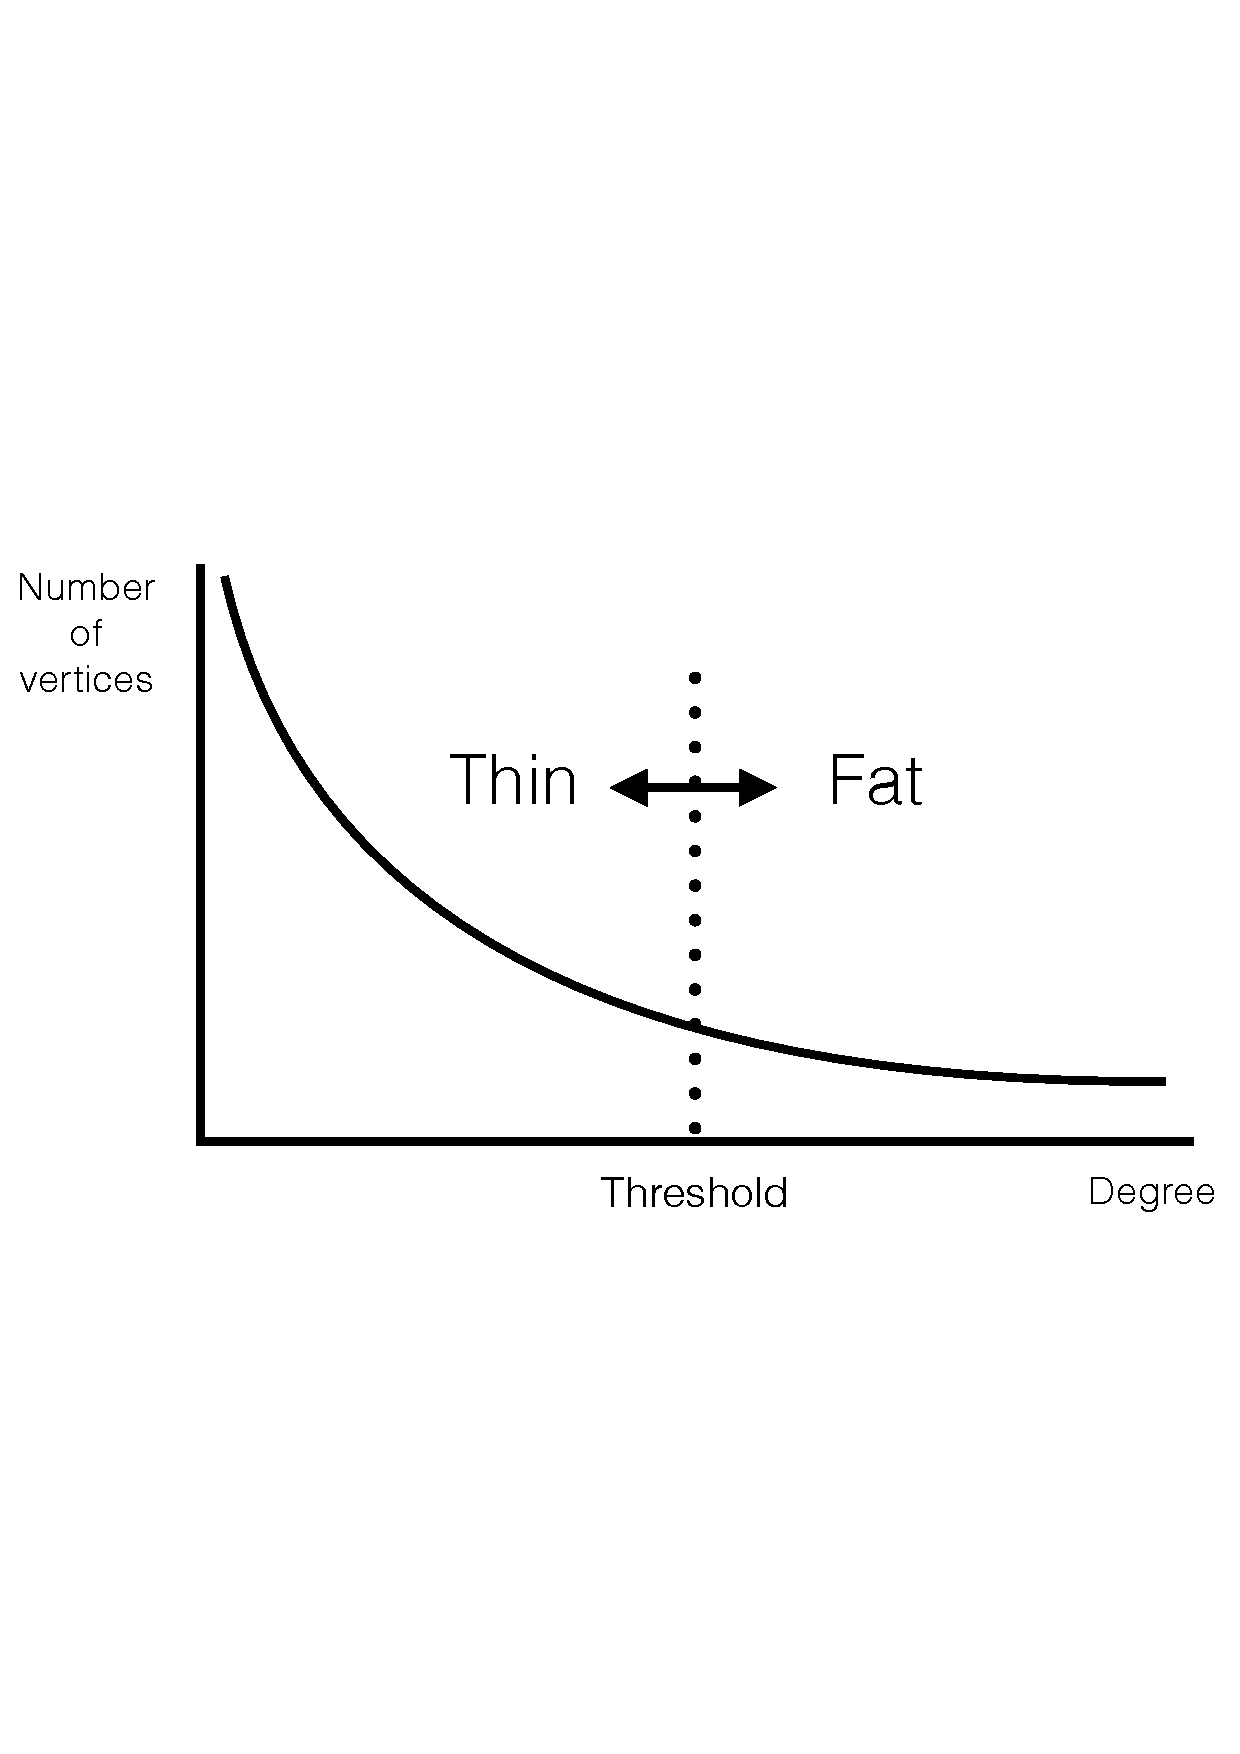
\includegraphics[width=0.23\textwidth]{Figures/Principle1.pdf}
}
\subfloat[]{
    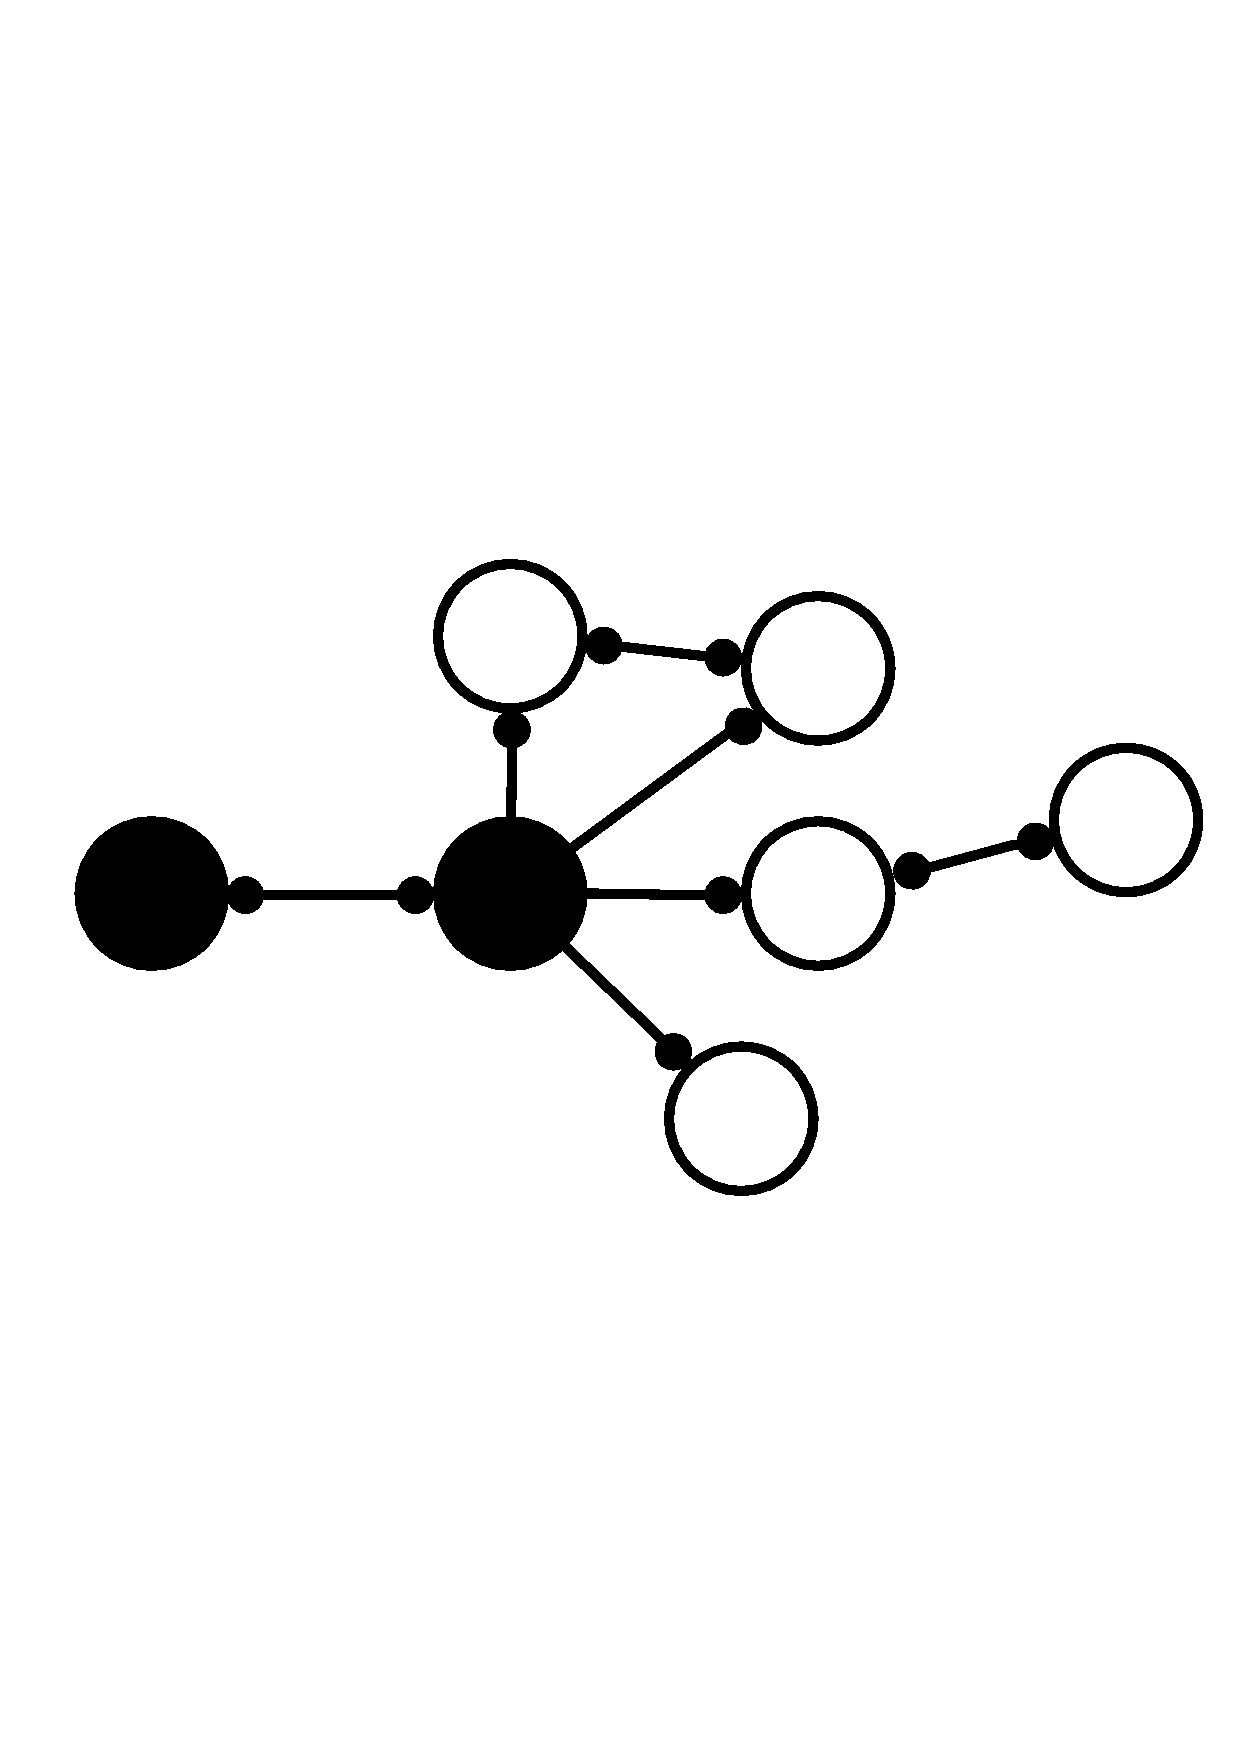
\includegraphics[width=0.23\textwidth]{Figures/Principle2.pdf}
}%(
\caption{Two illustrations of the main idea: Figure (a) demonstrates the threshold assignment, figure (b) demonstrates the label assignment, in which fat (black) nodes do not store adjacency to thin (white) nodes.}
    \label{f:principle}
\end{figure}

\subsection{Related work}
Adjacency labeling schemes for  numerous important graph families are by now well understood. 
general graphs  require a label size of $n/2+O(1)$~\cite{moon1965minimal, alstrup2014adjacency}, while 
trees, planar graphs, and bounded degree graphs enjoy labels of logarithmic size~\cite{Alstrup02, gavoille2007shorter, adjiashvili2014labeling}. 

Routing labeling schemes for power-law graphs  have been investigated by Brady and Cowen~\cite{brady2006compact}, and by Chen et al.~\cite{chen2012compact}. Labeling schemes for other properties than adjacency have been investigated for various classes of graphs, e.g., distance~\cite{gavoillea2004distance}, and flow~\cite{katz2004labeling}. 
Dynamic labeling schemes were studied by Korman and Peleg~\cite{korman2007general,korman2007compact,Korman07} and recently by Dahlgaard et. al~\cite{dahlgaard2014dynamic}.
Experimental evaluation for some labeling schemes for various properties on general graphs have been performed by Caminiti et.~al~\cite{caminiti2008engineering}, Fischer~\cite{fischer2009short} and Rotbart et.~al~\cite{rotbart2014evaluation}.

In the context of distributed graph computing systems,  a somewhat related paradigm of computation is the vertex centric computing model "think like a vertex". In this model  each vertex exchanges messages  only with nearby vertices, such that the locality and simplifies the design and implementation of such systems. Among the numerous systems proposed are Pregel~\cite{malewicz2010pregel}, Power-Graph~\cite{gonzalez2012powergraph} and GraphLab~\cite{low2012distributed}. For a recent survey on the topic see~\cite{mccunethinking2015}.






% !TEX root = Www.tex

\section{Preliminaries}
Throughout the paper we consider $n$-vertex, undirected, finite graphs.
For real $c > 0$, a graph is $c$-\emph{sparse} if it has at most $cn$ edges and \emph{sparse} if it is $c$-sparse for some constant $c$. For $0 < c \leq n-1$, the set of $c$-sparse graphs with $n$ vertices is denoted by $\Sparse$.
If $\mathcal{F}$ is a set of graphs,  $\mathcal{F}_n$ denotes the subset of graphs in $\mathcal{F}$ having exactly $n$
vertices. The degree of a vertex $v$ in a graph is denoted by $\Delta(v)$, and for non-negative integers $k$,
the set of vertices in a graph $G$ of degree $k$  is denoted by $V_k$.
The length of a binary string $x \in \{ 0,1 \}^*$ is denoted by $\vert x \vert$.
%We  denote the concatenation of two binary strings $x,y$  by $x \circ y$.

Let  $\mathcal{F}$ be a set of graphs. An  \emph{adjacency labeling scheme} (from hereon just \emph{labeling scheme}) for  $\mathcal{G}$
is a pair consisting of an \emph{encoder} and a \emph{decoder}. The encoder is an algorithm that receives $G \in \mathcal{G}$ as input and outputs a bit string $\la(v) \in \{0,1\}^*$ called the \emph{label} of $v$. The decoder 
is an algorithm that receives any two labels $\la(v),\la(u)$ as input and outputs $\mathtt{true}$ if{f} $u$ and $v$
are adjacent in $G$ and $\mathtt{false}$ otherwise. Note that the graph $G$ is not an input to the decoder.
The \emph{size} of a labeling scheme is the map $\textrm{size} : \mathbb{N} \longrightarrow \mathbb{N}$
such that $\textrm{size}(n)$ is the maximum length of any label assigned by the encoder to any vertex in
any graph $G \in \mathcal{F}_n$. The \emph{degree distribution} of a graph $G = (V,E)$ is the mapping
 $\mathrm{ddist}_G (k) : \mathbb{N}_0 \longrightarrow \mathbb{Q}$
defined by $\mathrm{ddist}_G (k) := \frac{\vert V_k \vert} {n}$.


%As the literature on power-law graphs usually allows some noise and deviation from the ``pure'' power-law distribution,  when devising our labeling scheme we consider a larger class of graphs, $\PLB$, that allows both a constant
%factor deviation from each point on the curve $k\mapsto Ck^{-\alpha}$ and an arbitrarily large deviation for small values of $k$. The class $\PLB$ subsumes the above ``ideal'' class $\PL$, whence our upper bounds on the size of labeling schemes hold for both $\PLB$ and $\PL$. Conversely, our lower bounds are proved on a very restrictive subclass $\PLC$ of $\PL$ whence the lower bounds hold for both $\PLC$ and $\PL$.



% !TEX root = WWW.tex

 \section{Power-Law Graphs}\label{Sec:GraphFamilies}

In the literature \emph{power-law} graphs are usually defined as the class of $n$ vertex graphs $G$ such that $\mathrm{ddist}_G(k)$
is proportional to $k^{-\alpha}$ for some real number $\alpha > 1$. Ideally, and ignoring rounding,  $\mathrm{ddist}_G(k) = Ck^{-\alpha}$ for all $k$ for constant $C$. As the degree distribution of a graph must be a probability distribution, we have $\sum_{k=1}^\infty C k^{-\alpha} = C \sum_{k=1}^\infty k^{-\alpha} = 1$, hence  $C = 1/\zeta(\alpha)$ where $\zeta$ is the Riemann zeta function. However, in the literature, concessions are usually made that relax
the restrictions on $\mathrm{ddist}_G(k)$, for example that the power-law property need only hold for high-degree
vertices (``above a cutoff''), or that $\mathrm{ddist}_G(k)$ is only \emph{approximately} equal to $Ck^{-\alpha}$,
with some approximation error that falls off with $n$.
To ensure that our results hold for all these variations of power-law graphs, 
 we define two families of graphs $\PLB$ and $\PLC$ with $\PLC\subsetneq\PLB$. Family $\PLB$ is rich enough to contain the graphs whose degree distribution is approximately, or perfectly, power-law distributed, and our upper bound on the label size for our labeling scheme holds for any graph in $\PLB$. Family $\PLC$ is used to show our lower bound
 and is restrictive enough that most definitions of power-law graph occurring in the literature will contain it. 
 
In the following, let $i_1 = \Theta(\sqrt[\alpha]n)$ be the smallest integer such that $\lfloor Cn/i_1^\alpha\rfloor \leq 1$, and let $C'\geq(\frac C{\alpha-1} + \frac{i_1}{\sqrt[\alpha] n} + 5)^{\alpha} + \frac{C}{\alpha - 1}$ be a constant; we shall use $C'$ in the remainder of the paper.
\begin{definition} \label{def:general-family}
Let $\alpha > 1$ be a real number and let $\chi:\mathbb N\rightarrow\mathbb N$ be a function. $\PLBARG{\chi}{\alpha}$ is the family of graphs $G$ such that if $n = \vert V(G)\vert$ then for all integers $k$ between $\chi(n)$ and $n-1$, $\sum_{i = k}^{n-1} {\vert V_i\vert} \leq C'(\frac{n}{k^{\alpha-1}})$. We shall usually suppress $\chi$ and $\alpha$, writing merely $\PLB$.
\end{definition}
The function $\chi$ captures the notion of a cutoff as defined in~\cite{clauset2009power} (Sec. 3.1); the intuition is  that for an $n$-vertex graph the power law distribution need only apply for nodes of degree higher than $\chi(n)$, rather than for all degrees. 
Setting $\chi(n) = 1$ corresponds to the case where the entire range of degrees follows a power-law distribution, hence
even for small values of $\chi(n)$, $\PLB$ morally contains all graphs with power-law degree distribution.
We will later prove upper bounds that hold for \emph{all} $\chi$ bounded from above by some function; in particular
for the upper bound for adjacency labelling schemes, the bound holds for $\chi(n)$ as high as  $\sqrt[\alpha]{n/\log n}$.

The class $\PLC$ contains graphs where  the number of vertices of degree $k$
must be $C \frac{n}{k^{\alpha}}$ rounded either up or down and the number of vertices of degree $k$ is non-increasing
with $k$. Note that the function $k \mapsto  C \frac{1}{k^{\alpha}}$ is strictly decreasing.

\begin{definition}\label{def:proper}
Let $\alpha > 1$ be a real number and let $C = 1/\zeta(\alpha)$ where $\zeta$ is the Riemann zeta function. $\PLCARG{\alpha}$ is the set of graphs  $G=(V,E)$ such that
\begin{enumerate}
\item $\lfloor Cn\rfloor - i_1 - 1\leq\vert V_1\vert\leq\lceil Cn\rceil$,
\item $\lfloor C\frac n{2^\alpha}\rfloor\leq\vert V_2\vert\leq\lceil C\frac n{2^\alpha}\rceil + 1$,
\item for every $i$ with $3 \leq i \leq n$:  $\vert V_i \vert\in \{\lfloor C\frac{n}{i^{\alpha}} \rfloor, \lceil C \frac{n}{i^{\alpha}} \rceil\}$, and
\item for every $i$ with $2 \leq i \leq n-1$: $\vert V_i \vert \geq \vert V_{i+1} \vert$.
\end{enumerate}
We usually suppress $\alpha$, writing just $\PLC$.
\end{definition}
Note that we allow slightly more noise in the sizes of $V_1$ and $V_2$ than in the remaining sets; without it, it seems tricky to prove a better lower bound than $\Omega(\sqrt[\alpha+1]{n})$ on label sizes.

We show the following properties of $\PLC$. 
%The proofs of Propositions~\ref{prop:powerlawsparse} and~\ref{prop:Contained} are in App.~\ref{App:GraphFamilies}.
\begin{proposition}\label{prop:maxvertexproper}\label{prop:maxdegree}
The maximum degree in an $n$-vertex graph in $\PLC$ is at most $\left(\frac{C}{\alpha - 1} + 2\right) \sqrt[\alpha]{n} + i_1 + 3 = \Theta(\sqrt[\alpha]n)$.
\end{proposition}

\begin{proof}
Let $n > 0$ be an integer and let $k' = \lfloor \sqrt[\alpha]{n} \rfloor$. 
Furthermore, let $S_{k'} = \sum_{i=1}^{k'} \vert V_i\vert$, that is $S_{k'}$ is the number of vertices of degree at most $k'$. Let $S^{-}_{k'} = (\sum_{i=1}^{k'} \lfloor Cni^{-\alpha}\rfloor) - i_1 - 1$. Then
$S_{k'} \geq S^{-}_{k'}$. We now bound $S^{-}_{k'}$ from below.
For every $i$ with $1 \leq i \leq k'$,
\begin{align*}
S^{-}_{k'} + k' & = -i_1 - 1 + \sum_{i=1}^{k'} \left(\left\lfloor Cn i^{-\alpha}\right\rfloor + 1\right) \geq \\ 
 &-i_1 - 1 + \sum_{i=1}^{k'} Cn i^{- \alpha}  = -i_1 - 1 + Cn \sum_{i=1}^{k'} i^{-\alpha} \\
    & \geq n \left(1 - C\sum_{i=k'+1}^{\infty} i^{-\alpha} \right) - i_1 - 1 \\
    & \geq n \left( 1 - C\int_{k'}^\infty x^{-\alpha} dx \right) - i_1 - 1\\
 & = n \left( 1 - C\left[ \frac{1}{\alpha - 1} x^{-\alpha + 1}\right]_{\infty}^{k'}\right) - i_1 - 1 \\
 & = n \left( 1 - \frac{C}{\alpha - 1} \left( \lceil\sqrt[\alpha]{n} \rceil \right)^{-\alpha + 1}\right) - i_1 - 1\\
 & \geq n \left( 1 -  \frac{C}{\alpha - 1} \left(\sqrt[\alpha]{n}\right)^{-\alpha + 1} \right) - i_1 - 1 \\
 & = n - \frac{Cn}{\alpha - 1}n^{-1+\frac{1}{\alpha}} - i_1 - 1\\
 & = n - \frac{C}{\alpha - 1}\sqrt[\alpha]{n} - i_1 - 1,
\end{align*}
giving $S_{k'} \geq S^{-}_{k'} \geq n - \frac{C}{\alpha - 1}\sqrt[\alpha]{n} - \lceil \sqrt[\alpha]{n} \rceil - i_1 - 1$. There are thus at most $\frac{C}{\alpha - 1} \sqrt[\alpha]{n} + \lfloor \sqrt[\alpha]{n} \rfloor + i_1 + 1$ vertices of degree strictly more than $k' = \lceil \sqrt[\alpha]{n} \rceil$. Since for every $1 \leq i \leq n-1$: $\vert V_i \vert \geq \vert V_{i+1} \vert$, it follows that the maximum degree of any graph in $\PLC$ is at most $\left(\frac{C}{\alpha - 1} + 2\right) \sqrt[\alpha]{n} + i_1 + 3$.
\end{proof}

\begin{proposition}\label{prop:powerlawsparse}
For $\alpha > 2$, all graphs in $\PLC$ are sparse.
\end{proposition}
\begin{proof}
By Proposition \ref{prop:maxvertexproper}, the maximum degree of an $n$-vertex graph in $\PLC$
graph is at most $k' \triangleq \left(\frac{C}{\alpha - 1} + 2\right) \sqrt[\alpha]{n} + i_1 + 3$, whence
the total number of edges is at most $\frac{1}{2}\sum_{k=1}^{k'} k \vert V_k\vert$. By definition,
$\vert V_k \vert\leq \lceil \frac{Cn}{k^\alpha}\rceil \leq \frac{Cn}{k^{\alpha}} + 1$ for $k\neq 2$ and $\vert V_2\vert\leq\lceil\frac{Cn}{2^{\alpha}}\rceil + 1$, and thus
\begin{align*}
\frac{1}{2}\sum_{k=1}^{k'} k\vert V_k\vert \leq 1 + \frac{1}{2}\sum_{k=1}^{k'} k \left(\frac{Cn}{k^{\alpha}} + 1 \right) \\
\leq 1 + \frac{k'(k'+1)}{4} + Cn\sum_{k=1}^{\infty} k^{-\alpha+1} \\
= O(n^{2/\alpha}) + Cn \zeta(\alpha - 1) = O(n).
\end{align*}
\end{proof}

\begin{proposition}\label{prop:Contained}
For any $\chi$ and $\alpha > 1$,
$\PLCARG{\alpha} \subseteq \PLBARG{\chi}{\alpha}$.
\end{proposition}
\begin{proof}
Let $d = \lfloor(\frac C{\alpha - 1} + 2)\sqrt[\alpha]{n} + i_1 + 3\rfloor$. For any graph in $\PLC$ with $n$ vertices and for any $k$, $\vert V_k\vert\leq Ck^{-\alpha}n + 1$ and by Proposition~\ref{prop:maxvertexproper}, $\vert V_k\vert = 0$ when $k > d$.

Let $k$ be an arbitrary integer between $\chi(n)$ and $n-1$. We need to show that $\sum_{i = k}^{n-1} {\vert V_i\vert} \leq C'(\frac{n}{k^{\alpha-1}})$. It suffices to show this for $k\leq d$. We have:
\begin{align*}
  \sum_{i = k}^{n-1} {\vert V_i\vert} & \leq \sum_{i = k}^d(Ci^{-\alpha}n + 1)=    d - k + 1 + Cn\sum_{i = k}^d i^{-\alpha}\\
  & \leq \left(\frac C{\alpha - 1} + \frac{i_1}{\sqrt[\alpha]n} + 5\right)\sqrt[\alpha]{n} + Cn\int_k^d x^{-\alpha}dx\\
  & \leq \left(\frac C{\alpha - 1} + \frac{i_1}{\sqrt[\alpha]n} + 5\right)\sqrt[\alpha]{n} + Cn\left[\frac 1{\alpha - 1}x^{-\alpha+1}\right]_\infty^k\\
  & \leq \left(\left(\frac C{\alpha - 1} + \frac{i_1}{\sqrt[\alpha]n} + 5\right)\left(\frac{\sqrt[\alpha]nd^{\alpha-1}}n\right) + \frac {C}{\alpha - 1}\right)nk^{-\alpha +1}\\
  & \leq \left(\frac C{\alpha - 1} + \frac{i_1}{\sqrt[\alpha]n} + 5\right)\left(\frac C{\alpha-1} + \frac{i_1}{\sqrt[\alpha]n} + 5\right)^{\alpha - 1}  nk^{-\alpha+1} \\
  & +  \left(\frac{C}{\alpha - 1}\right) nk^{-\alpha+1} \\
  & \leq C'nk^{-\alpha+1},
\end{align*}
as desired.
\end{proof}

\subsection{Comparison to other deterministic models}
Numerous probabilistic and  deterministic  definitions of power-law graphs are given in the literature.
A recent deterministic model, called  shifted power law distribution \cite{eom2011characterizing} has recently proven to capture a vast number of such definitions, both in theory and experimentally in \cite{Sankowski2016PowerLaw}.
We show that our definition of $\PLB$ contains graphs that adhere to the model, which is defined as follows.
 Let $c_1 > 0$ be a constant. A graph $G$ is \emph{power law bounded} for parameters $\alpha > 1$ and $t\geq 0$ if for every integer $d\geq 0$, the number of vertices of $G$ of degree in $[2^d,2^{d+1})$ is at most
\[
  c_1n(t+1)^{\alpha - 1}\sum_{i = 2^d}^{2^{d+1} - 1}(i+t)^{-\alpha}.
\]
As experimentally verified in \cite{Sankowski2016PowerLaw}, the value of $t$ is typically very small. If $t = O(1)$, the bound above becomes $O(n\sum_{i = 2^d}^{2^{d+1} - 1}i^{-\alpha})$. In this case, our family $\PLB(\chi,\alpha)$ is rich enough to contain these power law bounded graphs for sufficiently large $C'$ and any choice of $\chi$ and $\alpha$. This follows since for any power law bounded graph with $n$ vertices and any integer $k$ between $1$ and $n-1$, $\sum_{i = k}^{n-1}{\vert V_i\vert} = O(\sum_{d = \lfloor\lg k\rfloor}^{\lceil\lg(n-1)\rceil}n\sum_{i = 2^d}^{2^{d+1}-1}i^{-\alpha}) = O(\frac{n}{k^{\alpha-1}})$. Thus our upper bound also applies to power law bounded graphs. It is possible to extend our upper bound to super-constant $t$ where the bound is stronger the smaller $t$ is; we omit the details. Conversely, our family $\PLC$ is restrictive enough that
$\PLC$ is contained in the family of power law bounded graphs when $t = O(1)$, and the lower bound we derive thus
also holds in that setting.





% !TEX root = Main.tex

\section{The Labeling Schemes}
\label{sec:lab_schem}
We now construct algorithms for labeling schemes for $c$-sparse graphs and for the family $\PLB$. Both labeling schemes partition vertices into \emph{thin} vertices which are of low degree and \emph{fat} vertices of high degree. The \emph{degree threshold} for the scheme is the lowest possible degree of a fat vertex. We start with $c$-sparse graphs.
\begin{theorem}\label{sparse-label}
There is a $\sqrt{2cn\log n} + 2\log n + 1$ labeling scheme for $\Sparse$.
\end{theorem}
\begin{proof}
Let $G=(V,E)$ be an $n$-vertex $c$-sparse graph. Let $f(n)$ be the degree threshold for $n$-vertex graphs; we choose $f(n)$ below. Let $k$ denote the number of fat vertices of $G$, and assign each to each fat vertex a unique identifier between $1$ and $k$. Each thin vertex is given a unique identifier between $k+1$ and $n$.

For a $v\in V$, the first part of the label $\la(v)$ is a single bit indicating whether $v$ is thin or fat followed by a string of $\log n$ bits representing its identifier. If $v$ is thin, the last part of $\la(v)$ is the concatenation of the identifiers of the neighbors of $v$. If $v$ is fat, the last part of $\la(v)$ is a \emph{fat bit string} of length $k$ where the $i$th bit is $1$ iff $v$ is incident to the (fat) vertex with identifier $i$.

Decoding a pair $(\la(u),\la(v))$ is now straightforward: if one of the vertices, say $u$, is thin, $u$ and $v$ are adjacent iff the identifier of $v$ is part of the label of $u$. If both $u$ and $v$ are fat then they are adjacent iff the $i$th bit of the fat bit string of $\la(u)$ is $1$ where $i$ is the identifier of $v$.

Since $|E|\leq cn$, we have $k\leq 2cn/f(n)$. A fat vertex thus has label size $1 + \log n + k\leq 1 + \log n + 2cn/f(n)$ and a thin vertex has label size at most $1 + \log n + f(n)\log n$. To minimize the maximum possible label size, we solve $2cn/x = x\log n$. Solving this gives $x = \sqrt{2cn/\log n}$ and setting $f(n) = \lceil x\rceil$ gives a label size of at most $1 + \log n + (\sqrt{2cn/\log n} + 1)\log n\leq 1 + 2\log n + \sqrt{2cn\log n}$.
\end{proof}

%\begin{remark}\label{remark:FamilySize}
%It is easy to see that $f(n)$-sparse graphs enjoy a  $\sqrt{2f(n)} \log n$ %labeling scheme by setting the degree threshold to $\sqrt{2f(n)}$.
%In addition $c$-polysparse graphs enjoy a $n^{\frac{c}{2}} \log n$ labeling %scheme by setting the threshold to $n^{\frac{c}{2}}$.
%\end{remark}

By Proposition~\ref{prop:powerlawsparse}, graphs in $\PLC$ are sparse for $\alpha > 2$. This gives a label size of $O(\sqrt{n\log n})$ with the labeling scheme in Theorem~\ref{sparse-label}. We now show that this label can be significantly improved, by constructing a labeling scheme for $\PLB$ which contains $\PLC$.

\begin{theorem}\label{prop:labelingMain}
 There is a $\sqrt[\alpha]{C'n}(\log n)^{1 - 1/\alpha} + 2\log n + 1$ labeling scheme for $\PLB$.
\end{theorem}
\begin{proof}
The proof is very similar to that of Theorem~\ref{sparse-label}. We let $f(n)$ denote the degree threshold. If we pick $f(n)\geq \sqrt[\alpha]{n/\log n}$ then by Definition~\ref{def:general-family}  there are at most $C'n / f(n)^{\alpha -1}$ fat vertices. Defining labels in the same way as in Theorem~\ref{sparse-label} gives a label size for thin vertices of at most $1 + \log n + f(n)\log n$ and a label size for fat vertices of at most
$1 + \log n + C'n / f(n)^{\alpha -1}$.
We minimize by solving
$x \log n = C'n / x^{\alpha -1}$, giving $x = \sqrt[\alpha]{C'n/\log n}$. Setting $f(n) = \lceil x\rceil$ gives a label size of at most $\sqrt[\alpha]{C'n}(\log n)^{1 - 1/\alpha} + 2\log n + 1$.
\end{proof}
% !TEX root = WWW.tex
\subsection{A labeling scheme for random graphs}
There are schemes using randomness to ``grow''  graphs that, with high probability, have approximate power-law degree distribution for a range of degrees. One such scheme is the preferential attachment model \cite{barabasi1999emergence}. For graphs obtained from such models, their degree sequences are instead probability distributions. We now show that applying our labeling scheme for $\PLB$ to random graphs with the power law distribution results in a small expected worst-case label size.

Using the definition of Mitzenmacher \cite{mitzenmacher2004brief}, a random variable $X$ is said to have the \emph{power law} distribution (w.r.t.~$\alpha > 1$) if
\[
  Pr[X\geq x] \sim cx^{-\alpha+1},
\]
for a constant $c > 0$, i.e., $\lim_{x\to\infty}Pr[X\geq x]/cx^{-\alpha+1} = 1$.

Let $\epsilon > 0$ be fixed. Consider a graph $G$ picked from a family $\mathcal F$ of random graphs whose degree sequences have the power law distribution. Order the vertices of $G$ arbitrarily as $v_1,\ldots,v_n$. For $i=1,\ldots,n$, let indicator variable $X_i$ be $1$ iff $v_i$ has degree at least $d = \sqrt[\alpha]{n/\log n}$. There is a constant $N_0\in\mathbb N$ (depending on $\epsilon$) such that if $n\geq N_0$ then for all $i$,
\[
  E[X_i] = \mbox{Pr}[X_i = 1]\leq (1+\epsilon)cd^{-\alpha+1}.
\]

With the same labeling scheme as for $\PLB$ with degree threshold $\threshold{n} = d$, denote by $E_n$ the expected label size of an $n$-vertex graph from $\mathcal F$. Then for all $n\geq N_0$,
\begin{align*}
  E_n & = \sum_{x=0}^n \mbox{Pr}\left[\sum_{i=1}^n X_i = x\right]O((x+d\log n))\\
                       & = O\left(d\log n + E\left[\sum_{i=1}^n X_i\right]\right)\\
                       & = O\left(d\log n + \sum_{i=1}^n E[X_i]\right)\\
                       & = O\left(d\log n + nd^{-\alpha+1}\right)\\
                       & = O\left(\sqrt[\alpha]n(\log n)^{1-1/\alpha}\right).
\end{align*}
\begin{theorem}\label{th:random}
Let $\mathcal F$ be a family of graphs with degree sequences having the power law distribution w.r.t.~$\alpha > 1$. Then there is a labeling scheme for $\mathcal F$ such that the expected worst-case label size of any graph $G\in\mathcal F$ is $O(\sqrt[\alpha]n(\log n)^{1-1/\alpha})$ where $n$ is the number of vertices of $G$.
\end{theorem}


% !TEX root = WWW.tex

\section{Lower Bounds}
We now derive lower bounds for the label size of any  labeling schemes for both $\Sparse$ and  $\PLC$.
Our proofs rely on  Moon's~\cite{moon1965minimal} lower bound of  $\lfloor n/2 \rfloor$ bits for labeling scheme for general graphs.
We first show that the upper bound achieved for sparse graphs is close to the best possible.
The following proposition is essentially a more precise version of the lower bound suggested by Spinrad~\cite{spinrad2003efficient}.
\begin{proposition}
Any  labeling scheme for $\Sparse$ requires  labels of size at least $\left\lfloor\frac{\sqrt{cn}}2\right\rfloor$ bits.
\end{proposition}
\begin{proof}
Assume for contradiction that there exists a labeling scheme  assigning labels of size strictly less than $\lfloor\frac{\sqrt{cn}}2\rfloor$.
Let $G$ be an $n$-vertex graph. Let $G'$ be the graph resulting by adding $\left\lfloor\frac{n^2}{c}\right\rfloor - n$ isolated vertices to $G$, and note that now $G'$ is $c$-sparse. The graph $G$ is an induced subgraph of  $G'$.
It now follows that the vertices of $G$ have  labels of size strictly less than 
$\left\lfloor\frac{\sqrt{c\lfloor n^2/c\rfloor}}2\right\rfloor \leq n/2$ bits. As $G$ was arbitrary, we obtain a contradiction.
\end{proof}

\subsection{Lower bound for power-law graphs}
In the remainder of this section we are assuming that $\alpha>2$ and  prove the following:
\begin{theorem}\label{centralLowerBound}
For any $n$, any labeling scheme for $n$-vertex graphs of $\PLBARG{\chi}{\alpha}$ requires label size $\Omega(\sqrt[\alpha]{n})$.
\end{theorem}
More precisely, we present a lower bound for $\PLC$ which is contained in $\PLB$. Let $n\in\mathbb N$ be given and let $H = (V(H),E(H))$ be an arbitrary graph with $i_1$ vertices where $i_1 = \Theta(\sqrt[\alpha]n)$ is defined as in Section~\ref{Sec:GraphFamilies}. We show how to construct a graph $G = (V,E)$ in $\PLC$ with $n$ vertices that contains $H$ as an induced subgraph. Observe that a labeling of $G$ induces a labeling of $H$. As $H$ was chosen arbitrarily and as any labeling scheme for $k$-vertex graphs requires $\lfloor i_1/2 \rfloor$ label size in the worst case, Theorem~\ref{centralLowerBound} follows if we can show the existence of $G$.

We construct $G$ incrementally where initially $E = \emptyset$. Partition $V$ into subsets $V_1,\ldots,V_n$ as follows. The set $V_1$ has size $\lfloor Cn\rfloor - i_1$. For $i = 2,\ldots,i_1-1$, $V_i$ has size $\lfloor Cn/i^\alpha\rfloor$. Letting $n' = \sum_{i = 1}^{i_1-1} \vert V_i\vert$, we set the size of $V_i$ to $1$ for $i = i_1,\ldots,i_1+n-n'-1$ and the size of $V_i$ to $0$ for $i = i_1+n-n',\ldots,n$, thereby ensuring that the sum of sizes of all sets is $n$. Observe that $\sum_{i = 1}^{i_1}\lfloor Cn/i^\alpha\rfloor\leq n$ so that $n'\leq n - i_1$, implying that $n-n'\geq i_1$. Hence we have at least $i_1$ size $1$ subsets $V_{i_1},\ldots,V_{i_1+n-n'-1}$ in each of which the vertex degree allowed by Definition~\ref{def:proper} is at least $i_1$.

Let $v_1,\ldots,v_{i_1}$ be an ordering of $V(H)$, form a set $V_H\subseteq V$ of $i_1$ arbitrary vertices from the sets $V_{i_1},\ldots,V_{i_1+n-n'-1}$, and choose an ordering $v_1',\ldots,v_{i_1}'$ of $V_H$. For all $i,j\in\{1,\ldots,i_1\}$, add edge $(v_i',v_j')$ to $E$ iff $(v_i,v_j)\in E(H)$. Now, $H$ is an induced subgraph of $G$ and since the maximum degree of $H$ is $i_1-1$, no vertex of $V_i$ exceeds the degree bound allowed by Definition~\ref{def:proper} for $i = 1,\ldots,n$.

We next add additional edges to $G$ in three phases to ensure that it is an element of $\PLC$ while maintaining the property that $H$ is an induced subgraph of $G$. For $i = 1,\ldots,n$, during the construction of $G$ we say that a vertex $v\in V_i$ is \emph{unprocessed} if its degree in the current graph $G$ is strictly less than $i$. If the degree of $v$ is exactly $i$, $v$ is \emph{processed}.

\paragraph{Phase $1$}
Let $V' = V\setminus (V_1\cup V_H)$. Phase $1$ is as follows: while there exists a pair of unprocessed vertices $(u,v)\in V'\times V_H$, add $(u,v)$ to $E$.

When Phase $1$ terminates, $H$ is clearly still an induced subgraph of $G$. Furthermore, all vertices of $V_H$ are processed. To see this, note that the sum of degrees of vertices of $V_H$ when they are all processed is $O(i_1^2) = O(n^{2/\alpha})$ which is $o(n)$ since $\alpha > 2$. Furthermore, prior to Phase $1$, each of the $\Theta(n)$ vertices of $V'$ have degree $0$ and can thus have their degrees increased by at least $1$ before being processed.

\paragraph{Phase $2$}
While there exists a pair of unprocessed vertices $(u,v)\in V'\times V'$, add $(u,v)$ to $E$. At termination, at most one vertex of $V'$ remains unprocessed. If such a vertex exists we process it by connecting it to $O(\sqrt[\alpha]n)$ vertices of $V_1$; as $\vert V_1\vert = \Theta(n)$ there are enough vertices of $V_1$ to accomodate this. Furthermore, prior to adding these edges, all vertices of $V_1$ have degree $0$, and hence the bound allowed for vertices of this set is not exceeded.

\paragraph{Phase $3$}
We add edges between pairs of unprocessed vertices of $V_1$ until no such pair exists. If no unprocessed vertices remain we have the desired graph $G$. Otherwise, let $w\in V_1$ be the unprocessed vertex of degree $0$. We add a single edge from $w$ to another vertex $w'$ of $V_1$, thereby processing $w$ and moving $w'$ from $V_1$ to $V_2$. Note that the sizes of $V_1$ and $V_2$ are kept in their allowed ranges due to the first two conditions in Definition~\ref{def:proper}. This proves Theorem~\ref{centralLowerBound}.

% !TEX root = WWW.tex
\section{A distance labeling scheme}\label{Sec:Distance}
In this section we propose a distance labeling scheme for power law graphs. 

The \emph{distance} between two nodes in an undirected graph is the length of the shortest path connecting
the two nodes, if it exists, and $\infty$ if no such path exists.

Let $f : \mathbb{N} \longrightarrow \mathbb{N}$ be a map such that
$f(n) \leq  n -1$ for all $n$. An $f(n)$-\emph{distance labelling scheme} is a labelling
scheme such that, for any graph $G$, its decoder given labels $\mathcal{L}(u)$ and $\mathcal{L}(v)$ of two nodes $u$ and $v$
will output the distance between $u$ and $v$ if the distance is at most $f(\vert V(G) \vert)$, and output ``no'' if the distance
is  strictly greater than $f(\vert G \vert)$. If $f(n) = n-1$,
an $f(n)$distance labelling scheme is simply called a \emph{distance labelling scheme}.

For sparse graphs,
Alstrup et al.\ \cite{DBLP:journals/corr/AlstrupDKP15} obtain a distance labelling scheme with maximum label size
$O(\frac{n}{D} \log^2 D)$ where $D = (\log n)/(\log \frac{m+n}{n})$ and $m$ is the number of edges
in the graph.  Using similar methods, Gawrychowski et al.\ obtain an upper bond of \cite{DBLP:journals/corr/GawrychowskiKU15}
$O(\frac{n}{D} \log D)$ with sublinear decoding time. Few general results on lower bounds exist. The lower bound of $\Omega(\sqrt{n})$ for adjacency given in the present paper is trivially also a lower bound for distance; for total label size, the best known lower bound remains $\Omega(n^{3/2})$ as proved by Gavoille et al.~\cite{Gavoille2001}.

We now devise an $f(n)$-distance labelling scheme for $\PLBARG{C_2}$ working for any $C_2 \geq n^{1/(\alpha - 1 +f(n))}$.
The scheme has shorter labels than any known labelling schemes for small distances. As
the class of graphs with power law degree distribution is a subset of $\PLBARG{C_2}$, and as power-law graphs in general
have very small expected distances, the labelling scheme should work well for practical purposes in power-law graphs.

\begin{lemma}\label{lem:sparse_small_dist}
For any computable $f : \mathbb{N} \longrightarrow \mathbb{N}$ such that
$f(n) \leq n -1$ for all $n$, and for any $C_2 \geq \sqrt[\alpha-1+f(n)]{n}$ there is an $f(n)$-distance labelling scheme for $\PLBARG{C_2}$
that assigns labels of length at most $O(n^{f(n)/(f(n) + 1)} \log f(n))$.
\end{lemma}

\begin{proof}
As for adjacency labelling, the scheme is based on \emph{thin} and \emph{fat} nodes. Let $G$ be a graph
in $\PLBARG{C_2}$ Call
a node of $G$ \emph{fat} if it has degree at least $n^{1/(\alpha - 1 + f(n)}$ and \emph{thin} otherwise.
The label of each node $v$ now contains (i) a table of distances to all fat nodes (if the distance is more than $f(n)$, it is simply ignored), (ii) a table of distances to all thin nodes $w$ that are at most distance $f(n)$ away from $v$
where the shortest path between $v$ and $w$ does not pass through any fat node, and (iii) a single bit signifiying whether the node is fat or thin.
Clearly, as $f(n)$ is computable and distances in $G$ are computable, there is a computable encoder
assigning labels. A decoder can now compute the distance between any two nodes $u,v$ as follows:
If both $u$ or $v$ are fat, the distance can be directly read off part (i) of the label of any node. If at least one of $u$ 
and $v$ is fat, the distance can be read off part (i) of the label of the thin node. If both nodes are thin, the decoder
can check if the distance is in part (ii) of the label of either node; if the distance is not present, 
either the distance is strictly greater than $f(n)$, or the shortest path between $u$ and $v$ passes through
a fat node; in this case, the decoder may brute-force check the distances from $u$ and $v$ to each fat node,
and simply output the smallest sum of these two distances.

Furthermore, as all nodes of $G$ are either thin or fat, it is clearly possible for an encoder to compute
all distances less than or equal to $f(n)$ between any pair of nodes. Note that as all distances we care for 
are bounded above by $f(n)$, each such distance can be stored using at most $\log f(n)$ bits.

As $G = G(V,E)$ is in $\PLCARG{C_2}$, we have 
\begin{align*}
\sum_{i = C_2}^{n-1} \vert V_i \vert
&\leq \sum_{i = n^{\frac{1}{\alpha - 1 + f(n)}}}^{n-1} \vert V_i \vert \leq C' \left( \frac{n}{\left( n^{\frac{1}{\alpha - 1 + f(n)}}\right)^{\alpha - 1}}\right)\\
&\leq C' n^{1 - (\alpha - 1)/{\alpha-1 + f(n)}} 
= C' n^{f(n)/(\alpha - 1 + f(n))}
\end{align*}
 Thus, a table of distances to all fat nodes takes up at most $O\left(n^{\frac{f(n)}{\alpha - 1 + f(n)}} \log f(n)\right)$ bits.

Similarly, for each node $v$ there are at most $\left(n^{1/(\alpha - 1 + f(n))}\right)^{f(n)} = n^{f(n)/(\alpha - 1 + f(n))}$ nodes at distance at most $f(n)$ away from $v$ where the shortest path consists only of thin nodes. Hence, the associated table of distances
takes up at most \\$O(n^{f(n)/(\alpha -1 + f(n))} \log n)$ bits.

In total, each label thus has size at most $O(n^{f(n)/(f(n)+1)} \log n)$ bits.
\end{proof}

For $f(n) = \log n$, Lemma \ref{lem:sparse_small_dist} yields a labelling scheme having label size
at most $O\left(n^{(\log n)/(\alpha - 1 + \log n)} \log\log n \right)$. Unsurprisingly, as we are only considering distances up
to $f(n)$, this label size is asymptotically smaller than for the labelling
schemes working for all distances in \emph{sparse} graphs, e.g. the largest label sizes of \cite{DBLP:journals/corr/GawrychowskiKU15} for sparse graphs is $O(n \frac{\log \log n}{ \log n})$.
For power law random graphs, Chung and Lu show in \cite{chung2004average} that, subject to mild conditions, the diameter of power law graphs with $\alpha > 2$ is almost surely $\Theta(\log n)$. We thus expect our labelling scheme to have
superior performance for such graphs.
% !TEX root = WWW.tex
\subsection{Scale Free  Graphs from Generative Models}\label{Sec:ScaleFree}
%In this section we treat the generative  BA model, conjectured to create power-law graphs\footnote{
%Bollobas~\cite{bollobas2003mathematical}(Sec. 6 and 7) proved that for a similar model vertices of degree smaller than $\sqrt[15]{n}$ in fact abide a power-law distribution. }.
The Barab{\'a}si-Albert (BA) model is a well-known generative model for power-law graphs that, roughly, grows a graph in a sequence of time steps by
inserting a single vertex at each step and attaching it to $\mathcal{E}$ existing vertices with probability weighted by the degree of each existing vertex \cite{barabasi1999emergence}. The BA model
generates graphs that asymptotically have a power-law degree distribution ($\alpha = 3$) for low-degree nodes \cite{DBLP:journals/rsa/BollobasRST01}.
Graphs created by the BA model have low arboricity \footnote{the arboricity of a graph is the minimum number of spanning forests needed to cover its edges.}~\cite{goel2006bounded} we use
that fact to prove the following highly efficient labeling scheme. 

\begin{proposition}\label{Th:baLabeling}
The family of graphs generated by the BA model has an $O(\mathcal{E} \log n)$ adjacency labeling scheme.
\end{proposition}

\begin{proof}
Let  $G=(V,E)$  be an $n$-vertex graph resulting by the construction  by the BA model with some parameter $m$ (starting from some graph $G_0 = (V_0,E_0)$ with $\vert V_0 \vert \ll n$).
While it is not known how to compute the   arboricity of a graph efficiently, it is possible in near-linear time to compute a partition of $G$ with  at most twice\footnote{More precisely, for any $\epsilon \in (0,1)$  there exist an $O(|E(G)| / \epsilon)$ algorithm~\cite{kowalik2006approximation} that computes such partition using at most $(1+ \epsilon)$ times more forests than the optimal.} the number of forests in comparison to the optimal~\cite{arikati1997efficient}.
We can thus decompose the graph to $2\mathcal{E}$ forests in near linear time and label each forest using the recent $\log n + O(1)$ labeling scheme for trees~\cite{alstrup2015optimal},  and achieve a $2\mathcal{E} (\log n+O(1))$ labeling scheme for $G$.
\end{proof}

Note that if the encoder operates at the same time as the creation of the graph, Proposition \ref{Th:baLabeling} can be strengthened to yield  an $m \log n$ labeling scheme: simply store the  
 identifiers of the $m$ vertices attached with every vertex insertion.
Theorem~\ref{centralLowerBound} and Proposition \ref{Th:baLabeling} strongly suggest that, for each sufficiently large $n$, the number of  power-law graphs with $n$ vertices  is vastly larger than the number of graphs with $n$ vertices created by the  BA model.  In contrast, other generative models such as   Waxman~\cite{waxman1988routing}, N-level Hierarchical~\cite{calvert1997modeling}.
and Chung's~\cite{chung2006complex} (Chapter 3)  do not seem to have an obvious smaller label size than the one in Proposition~\ref{prop:labelingMain}.

% !TEX root = WWW.tex
\section{Experimental Study}

We now  perform an experimental evaluation of our labeling scheme on a number of real-world networks.
Source code for our experiments can be found at:\\ \url{www.diku.dk/~simonsen/suppmat/www16/powerlaw.zip}

\subsection{Experimental Framework}\label{Sec:Experimental}
Recall that our labeling scheme separates  the nodes according to a selected threshold from the range $0$ to the maximal degree $\Delta$ of a node in the graph. The threshold is selected as a function of  the power-law parameter $\alpha$.
The following observation is the key to assess our labeling scheme's quality.
Suppose we chosoe a threshold  $n_0$ for a graph $G$. Call  the maximum label size thin and fat nodes $T(n_0)$ and $F(n_0)$ respectively. Then, the maximum label assigned by our labelling scheme-hence the quality of the scheme--is the larger of these two values.
The critical observation is that, as our selection of threshold $n_0$ increases, $T(n_0)$ monotonically increases and  $F(n_0)$ monotonically decreases.
The optimum value of $n_0$ is thus the one that minimises  $F(n_0)-T(n_0)$, in other words, where the graphs of
the functions $T(\cdot)$ and $F(\cdot)$ intersect.
In the remainder of this section we call this optimum threshold the \emph{empirical} threshold.For large real-world graphs, computing the empirical threshold requires operations on the entire network: a slow encoder for a labeling scheme can always find the empirical threshold by a binary search, but this would incur an $O(\log n)$ factor on its running time. 

In contrast, we set the threshold in our labeling scheme as $\lceil \sqrt[\alpha]{C n/(\alpha-1)} \rceil$, which we denote as the \emph{predicted} threshold. The predicted and the empirical threshold will be identical when the degree distribution of the data perfectly follows a power-law curve with parameter $\alpha$. As real-world data rarely follow a power-law
graph perfectly, there could conceivably be substantial difference between the predicted and the empirical threshold.


\paragraph{Performance Indicators}
We use the following to determine the quality of our labeling scheme:

\emph{Performance Indicator i:} We  compare the label sizes attained by our labeling schemes to other labeling schemes, namely state-of-the art labeling schemes for the classes of bounded-degree, sparse and general graphs using the  labeling schemes suggested in \cite{adjiashvili2014labeling},  Theorem~\ref{sparse-label} and \cite{alstrup2014adjacency}.  We interpret small label sizes for our scheme, especially in comparison with ``small'' classes like the class of bounded-degree graphs, as a sign that our labeling scheme efficiently utilizing  the extra information about the graphs: namely that their degree distribution is reasonably well-approximated by a power-law.

\emph{Performance Indicator ii:} We measure the difference in label sizes using the predicted and empirical thresholds. 
 We also measure  the difference between the predicted and empirical threshold in percentages with respect to the maximum degree.
We interpret a small relative differences in those as an evidence  that the predicted threshold can achieve small label sizes without examining the global properties of the network other than the power-law parameter $\alpha$. 
This best captures how close our ''guess" of the right threshold was, and will, in practice, allow for a faster encoding time.
 




 
 %\footnote{Additional notes on these values are found in Appendix~\ref{Section:TotalStorage}.

\paragraph{Test Sets}
We employ both real-world and synthetic data sets. 

The six \emph{synthetic} data sets are created by first generating a power-law degree sequence using the method of Clauset et al.~\cite[App.\ D]{clauset2009power}, subsequently constructing a corresponding graph for the sequence using the Havel-Hakimi method~\cite{hakimi1962realizability}. 
We use the range $2< \alpha < 3$ as suggested in~\cite{clauset2009power} as this range of $\alpha$ occurs most commonly in modeling of real-world networks. We generate graphs of $300,000$ and $1M.$ vertices denoted  s300$^{\alpha=x}$  and s1M$^{\alpha=x}$  respectively, for $x \in \{2.2,2.4,2.6,2.8\}$. 


The seven \emph{real-world} data sets originate  from articles that found the data to be well-approximated by a power-law. 
The \textsc{www} data set  \cite{albert1999internet} contains information on links between webpages within the nd.edu domain. 
The \textsc{enron} data set ~\cite{leskovec2009community}  contains email communication between  Enron employees (vertices are email addresses; there is a link between two addresses
if a mail has been sent between them).
The \textsc{internet} data set~\cite{newman} provides a snapshot the Internet structure at the level of  autonomous systems, reconstructed from BGP tables. 
For all of these sets, we consider the underlying simple, undirected graphs. For each set, standard maximum likelihood methods were used to compute the parameter
$\alpha$ of the best-fitting power-law curve \cite{clauset2009power}. Additional information on the data sets can be found in Table~\ref{t:datasets}.

\begin{table}[!ht]
\centering
\small
\begin{tabular}{lccccl}\hline
\multicolumn{6}{c}{Real-Life Graphs}\\\hline
Data set  & $\vert V \vert$ & $\vert E\vert$ & $\alpha$  & $\Delta_{\max}$ & Source\\\hline
\textsc{internet} &  22,963        &    48,436      & 2.09     & 2,390        & \cite{newman}\\
\textsc{enron}    &  36,692        &   183,830      & 1.97    &1,383         & \cite{leskovec2009community}\\
\textsc{www}      & 325,729        & 1,117,563     & 2.16 & 10,721            & \cite{albert1999internet}\\
\textsc{google} & 875,713 & 5,105,039 & 2.73 & 6,332 & \cite{leskovec2009community}\\
\textsc{Youtube} & 1,134,890 & 2,987,624 & 2.14 & 28,754 & \cite{yang2015defining}\\
\textsc{wikitalk} & 2,394,385 & 5,021,410 & 2.42 & 100,032 & \cite{leskovec2010predicting}\\
\textsc{LiveJournal} &  3,997,962        &    34,681,198      & 2.97     & 14,815        & \cite{yang2015defining}\\\hline


\multicolumn{6}{c}{Synthetic Graphs}\\\hline
s300$^{\alpha=2.2}$    & 300,000        & 491,926        & 2.2    & 10,906 & --\\
s300$^{\alpha=2.4}$    & 300,000        & 327,631        & 2.4    & 3,265 & --\\
s300$^{\alpha=2.6}$    & 300,000        & 261,949        & 2.6    & 1,410 & --\\
s300$^{\alpha=2.8}$    & 300,000        & 227,247        & 2.8    & 1,842 & --\\
s1M$^{\alpha=2.4}$    & 1,000,000       & 1,127,797      & 2.4    & 42,683 &-- \\
s1M$^{\alpha=2.6}$    & 1,000,000       & 878,472        & 2.6    & 12,169 &-- \\
s1M$^{\alpha=2.8}$    & 1,000,000       & 751,784         & 2.8   & 1,692  &-- \\\hline
\end{tabular}
\caption{Data sets and their properties. All graphs are undirected and simple. $\Delta_{\max}$ is the maximum degree of any vertex in the data set.}
\label{t:datasets}
\end{table}


\subsection{Findings}
Figure \ref{fig:findings} shows the distribution of maximum label sizes for two representative synthetic and  data sets. The maximum label size
for the predicted and empirical thresholds as well as upper bounds on the label sizes from different label schemes in the literature can be seen in Table \ref{t:labelsizes}. 
%Plots for the remaining data sets can be found in Appendix~\ref{App:ExpRes}.

\begin{figure*}[!ht]
\centering
\subfloat[\small s300$^{\alpha=2.2}$]{
    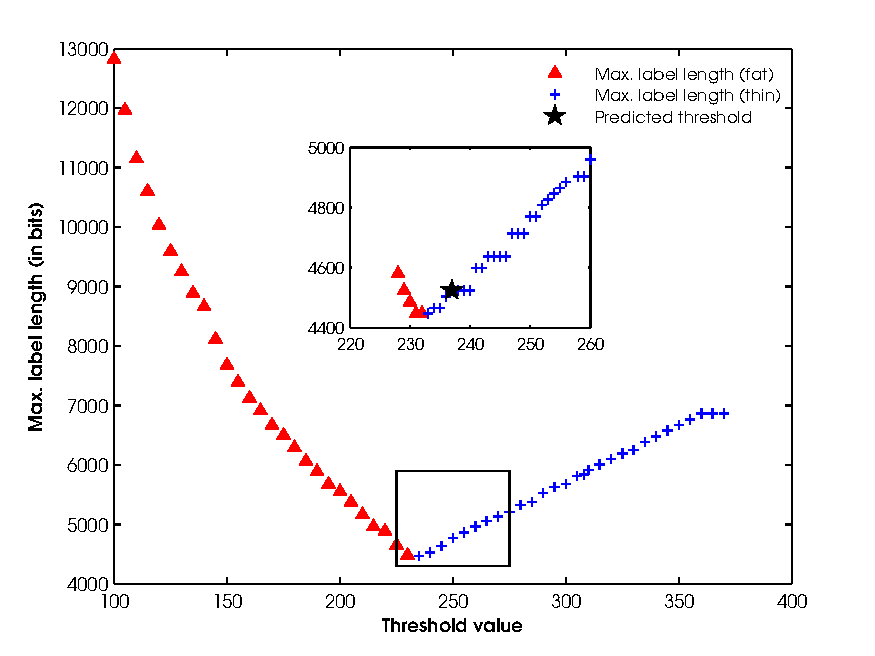
\includegraphics[width=0.3\textwidth]{Figures/synthetic-300k-alpha22.pdf}
    \label{f:fsyn300k}
}\hspace*{-2.5em}
\subfloat[\small \textsc{\small s1M$^{\alpha=2.6}$}]{
    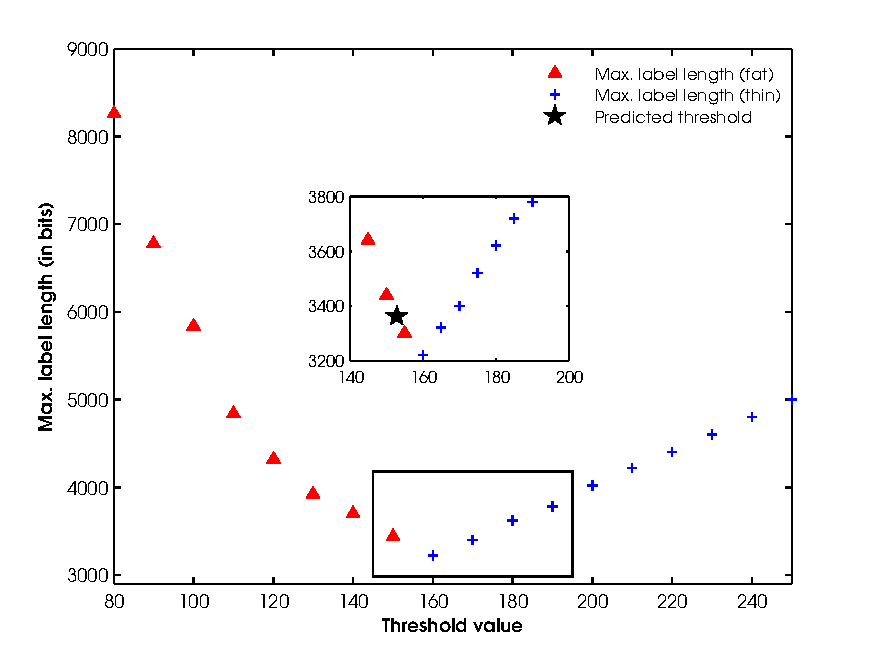
\includegraphics[width=0.3\textwidth]{Figures/synthetic-1M-26}
    \label{f:fsyn1M}
}%
\caption{Exemplary maximum label sizes of different threshold values for the synthetic data sets   s300$^{\alpha=2.2}$ and s1M$^{\alpha=2.6}$. 
The triangles and crosses represent that for the tested threshold the largest label belong to fat, resp. thin node. The star indicate the position of the predicted threshold.
See~\cite{} for the remaining  figures for synthetic datasets.}
\label{fig:findings}%
\end{figure*}

% !TEX root = WWW.tex
\begin{figure*}[!ht]
\centering
\subfloat[\small Fat and thin vertices vs. threshold values]{
    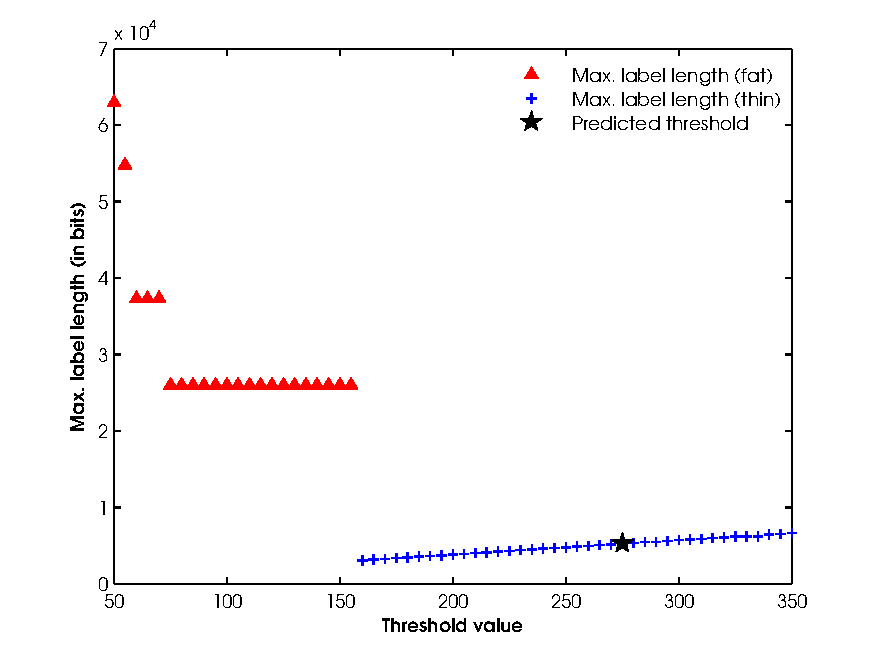
\includegraphics[width=0.4\textwidth]{Figures/barabasi-www.pdf}
}
\subfloat[\small Power law fit]{
    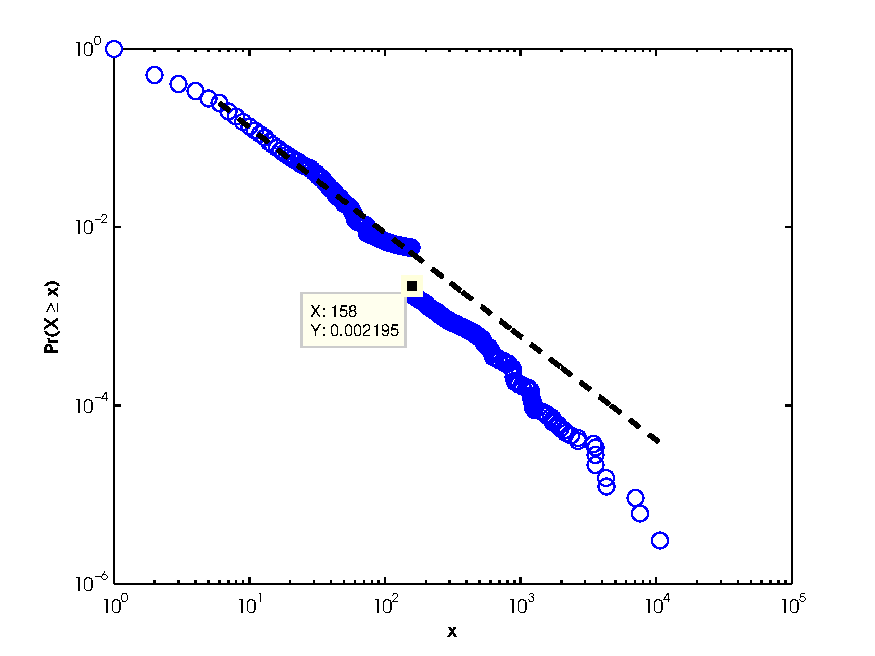
\includegraphics[width=0.4\textwidth]{Figures/barabasi-www-ccdf.pdf}
}%
\quad
\subfloat[\small Fat and thin vertices vs. threshold values]{
    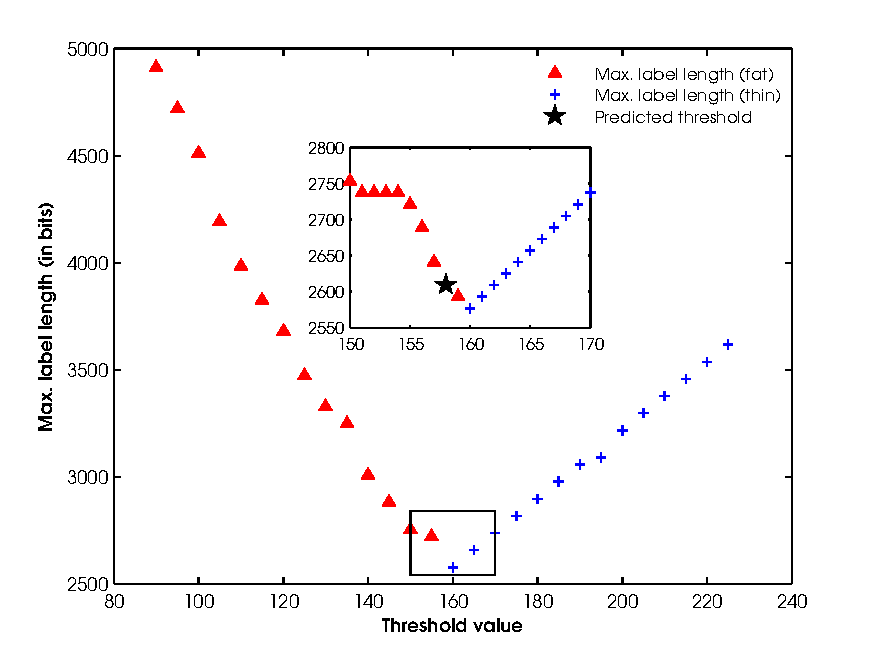
\includegraphics[width=0.4\textwidth]{Figures/enron-mail.pdf}
}
\subfloat[\small Power law fit]{
    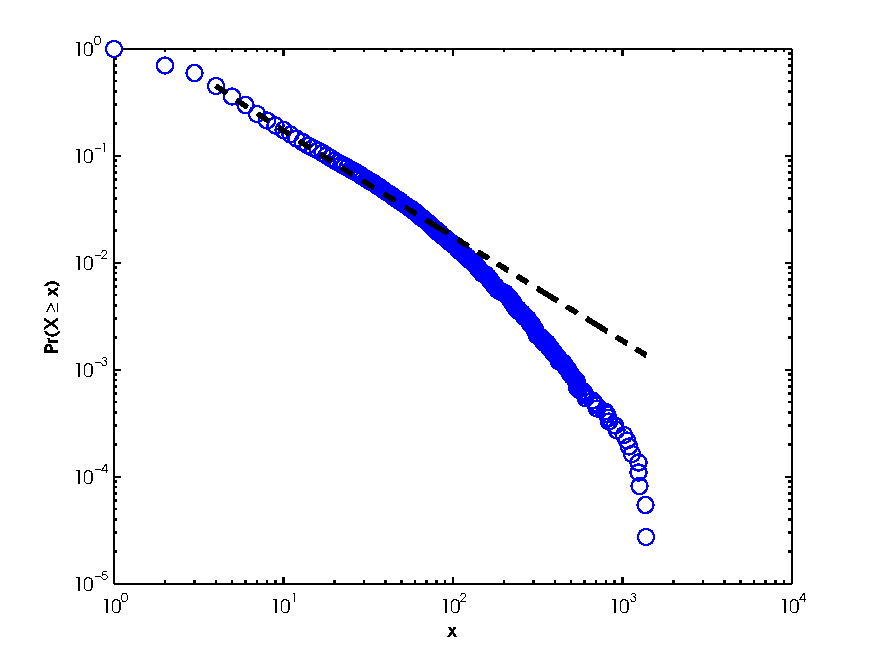
\includegraphics[width=0.4\textwidth]{Figures/enron-mail-ccdf.pdf} 
}%
\quad
\subfloat[\small Fat and thin vertices vs. threshold values]{
    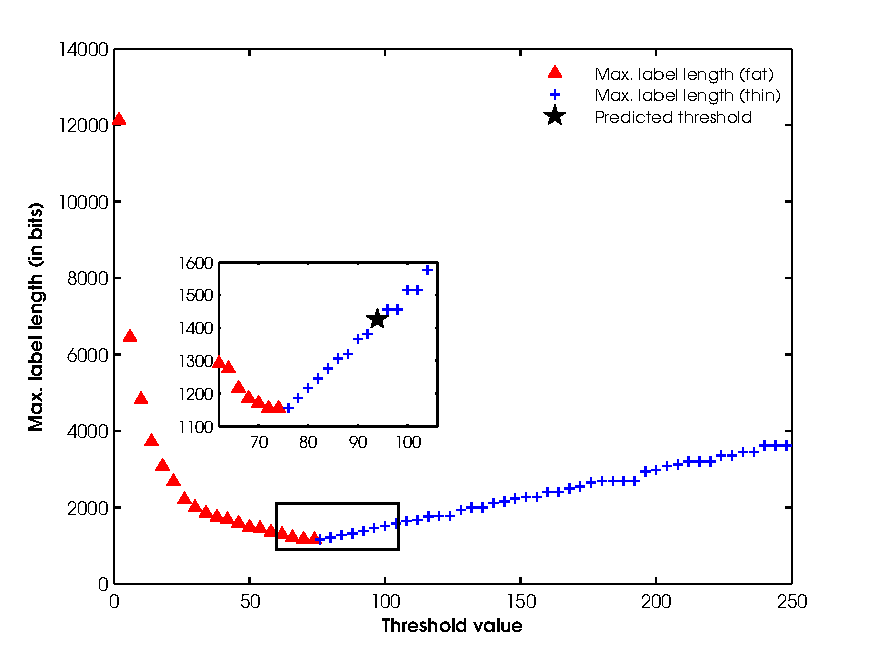
\includegraphics[width=0.4\textwidth]{Figures/internet.pdf}
}
\subfloat[\small Power law fit]{
    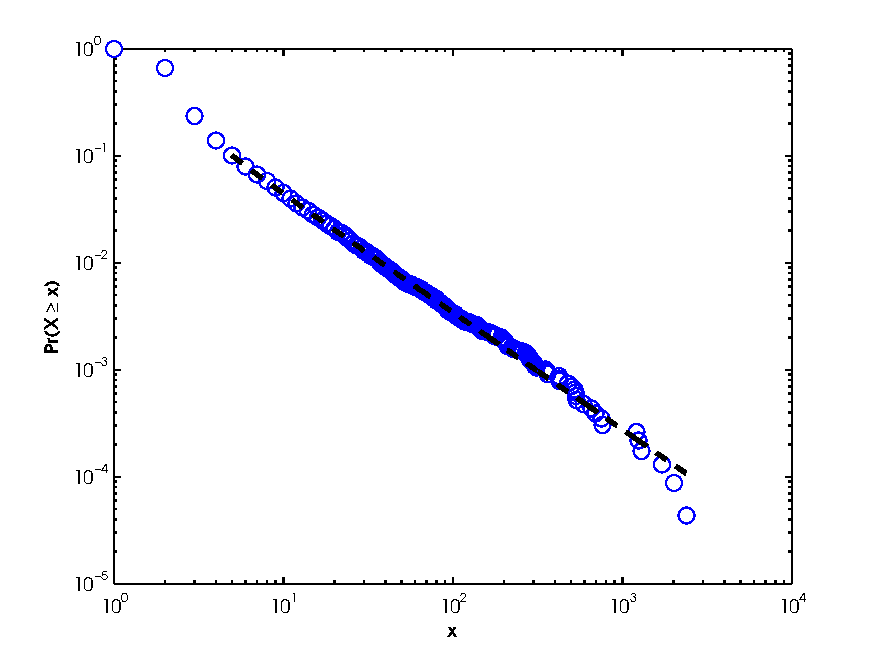
\includegraphics[width=0.4\textwidth]{Figures/internet-ccdf.pdf}
}%
\caption{Left: Fat and thin vertices plotted against increasing threshold values for the \textsc{enron} email communication dataset. The black pentagram is the predicted threshold ($1/\zeta(\alpha)\sqrt[\alpha](n)$) rounded to the nearest integer.  Right: Best-fitting power law ($\alpha = 1.97$)  superimposed on the complementary cumulative distribution function (CCDF) using the framework by \cite{clauset2009power}.}%
\label{fig:synthetic300}%
\end{figure*}
% !TEX root = WWW.tex
\begin{figure*}[!ht]
\centering
\subfloat[\small \textsc{enron}]{
    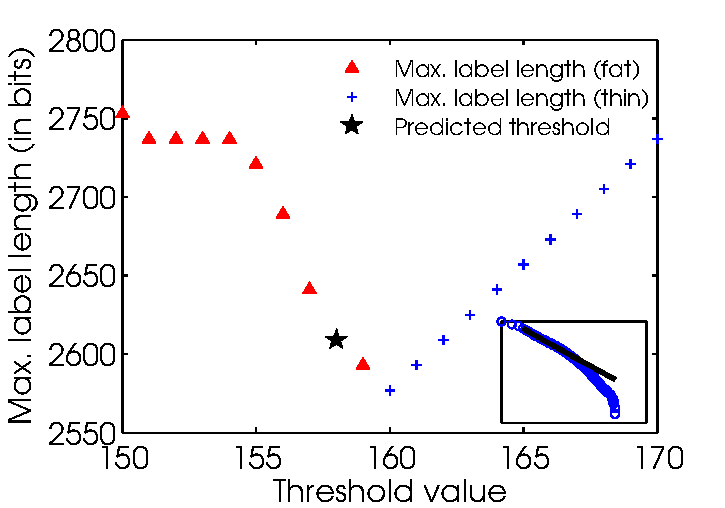
\includegraphics[width=0.32\textwidth]{Figures/enron-modified.pdf}
}
\subfloat[\small \textsc{internet}]{
    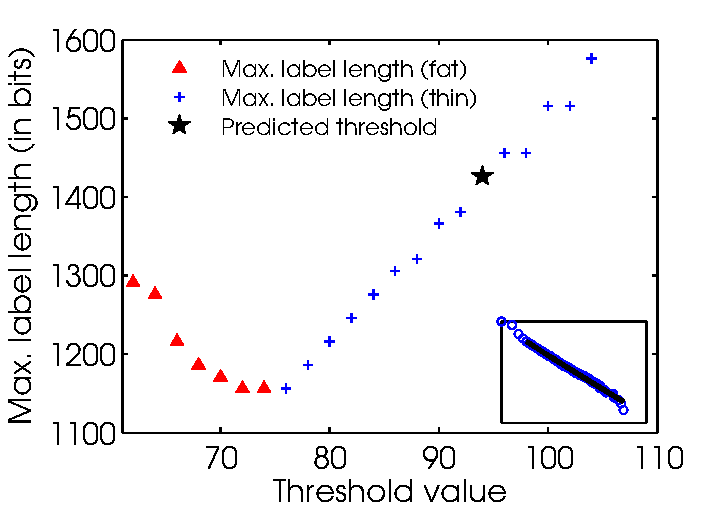
\includegraphics[width=0.32\textwidth]{Figures/internet-modified.pdf}
}%
\subfloat[\small \textsc{www}]{
    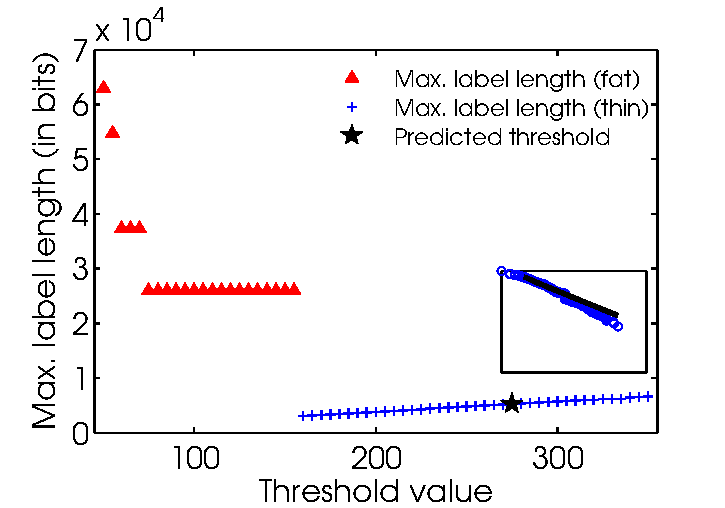
\includegraphics[width=0.32\textwidth]{Figures/www-modified.pdf}
}%
\caption{Predicted and empirical thresholds for the \textsc{enron}, \textsc{internet} and \textsc{www} datasets. The inset show the MLE fitted power law, using the method of Clauset et al.\ \cite{clauset2009power}, where data points are blue circles and the power law is shown as a black solid. The exponents of the power laws are shown in Table \ref{t:data sets}.}%
\label{f:bla}%
\end{figure*}
% !TEX root = WWW.tex
\begin{figure}[!ht]
\centering
\hspace*{-1em}
\subfloat[\small s300$^{\alpha=2.2}$]{
    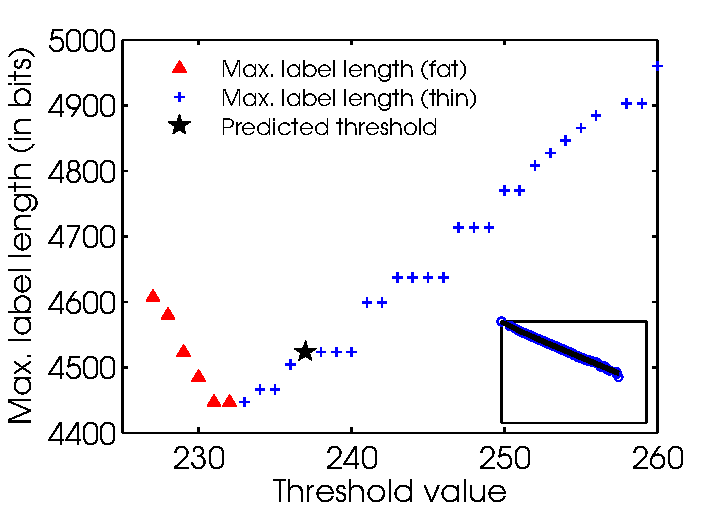
\includegraphics[width=0.55\columnwidth]{Figures/synthetic-data-300K-alpha22-revised.pdf}
}\hspace*{-1.9em}
\subfloat[\small s1M$^{\alpha=2.6}$]{
    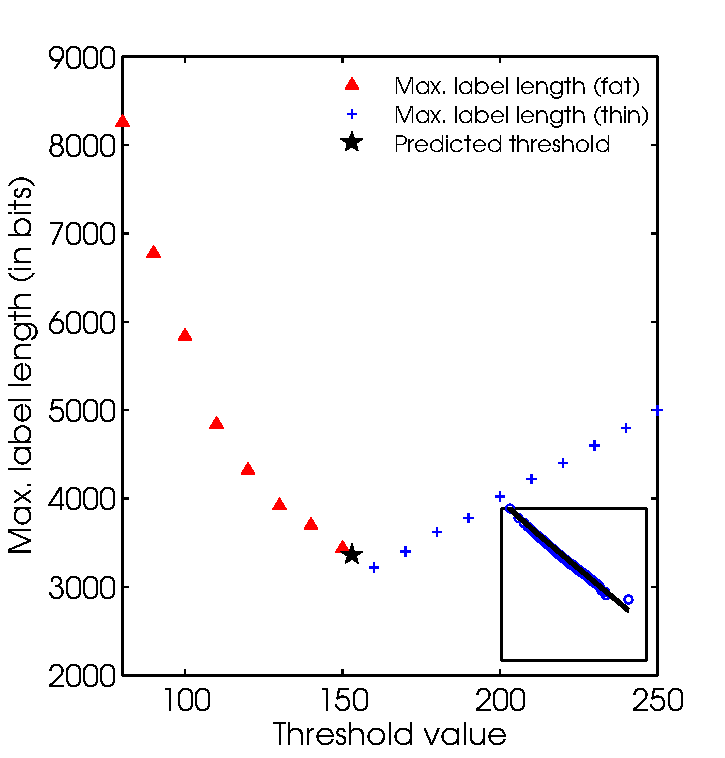
\includegraphics[width=0.55\columnwidth]{Figures/synthetic-data-1M-alpha26-revised.pdf}
}%
\caption{Exemplary maximum label sizes of different threshold values for the synthetic data sets s300$^{\alpha=2.2}$ and s1M$^{\alpha=2.6}$. 
The triangles and crosses represent that for the tested threshold the largest label belong to fat, resp. thin node. The star indicate the position of the predicted threshold.
See~\cite{} for the remaining  figures for synthetic datasets.}%
\label{f:bla}%
\end{figure}

Table~\ref{t:labelsizes}  shows  the maximum label sizes achieved using different labeling schemes on our data sets. ``Predicted'' shows the experimental maximum label size obtained by running our scheme on the graphs, ``Empirical'' is the label size attained by using the empirical threshold.
``Label Diff.'' shows the ratio between the predicted and empirical label sizes, and  ``Threshold Diff.'' shows the ratio between the absolute difference of the threshold values and the maximum degree.
 The remaining columns show non-experimental upper bounds for different label schemes: ``Bound'' is the upper bound guaranteed in Theorem~\ref{prop:labelingMain}, ``$c$-sparse'' is  the labeling scheme for sparse graphs defined in Theorem~\ref{sparse-label}, ``BD'' is the $\lceil \frac{\Delta}{2} \rceil \lceil \log n\rceil$ bounded degree graph  labeling of~\cite{adjiashvili2014labeling}, and AKTZ is the $\lceil n/2\rceil+6$ general graph  labeling of~\cite{alstrup2014adjacency}.
 
For the dataset groups ``Real-Life" and ``Synthetic", the values of  ``Empirical'' and  ``Bound'' are represented using simple concatenation of labels to represent both the fat and thin bit strings. 
In comparison to our analysis, this may incur a factor of up to $(\log n)/\alpha$  on the fat nodes and discount a similar factor for the thin nodes.
Due to the size of the datasets in the group  "Real-Life Large Graphs", the computation of their predicted and empirical bounds was done using the observation that in our original labeling scheme the following holds: Given a  graph $G=(V,E)$, and threshold $t$, with $v_t \in V$ nodes of degree larger than $t$, the label size is $\max{(v_t,t \log n)}$. 

\begin{table*}
\small
\begin{tabular}{ccccccccc}
\hline \multicolumn{9}{c}{Real-Life Graphs}\\\hline
Data set&Predicted &Empirical & Label Diff. & Threshold Diff.   & Upper-Bound     &$c$-sparse &Bounded Degree \cite{adjiashvili2014labeling} &AKTZ \cite{alstrup2014adjacency}\\\hline
\textsc{internet}   &$1,426$    &$1,156$  & $19.0\%$  & $0.8\%$  & $8,181 $  &$4,700$      &$17,925$  &$11,487$\\
\textsc{enron}      &$2,609$    &$2,577$  & $1.3\%$ & $0.2\%$   & $15,835 $ &$9,735$      &$11,056$  &$18,352$\\
\textsc{www}        &$5,245$    &$3,060$  & $41.7\%$  & $1\%$  & $29,225 $ &$28,445$     &$101,840$ &$162,870$ \\
\hline \multicolumn{9}{c}{Real-Life Large Graphs}\\\hline
\textsc{google} & $3,421$ & $2,617$ & $131\%$ & $0.2\%$ & $6,381$ & $23,568$ & $63,320$ & $437,863$\\
\textsc{Youtube}        &$10,596$    &$3,212$  & $329\%$  & $1.3\%$  & $21,7190$ &$25,872$     &$301,917$ &$578,920$ \\
\textsc{WikiTalk}       & $6,972$ & $4,282$ & $162\%$ & $0.1\%$ & $16,664$ & $41,110$ & $1,100,330$ & $1,197,199$\\ 
\textsc{LiveJournal}        &$62,878$    &$7,874$  & $798\%$  & $1.6\%$  & $8,279$ &$56,644$     &$162,976$ &$1,998,987$ \\\hline
\multicolumn{9}{c}{Synthetic Graphs}\\\hline
Data set&Predicted &Empirical & Label Diff. & Threshold Diff.   & Upper-Bound     &$c$-sparse &Bounded Degree \cite{adjiashvili2014labeling} &AKTZ \cite{alstrup2014adjacency}\\\hline
s1M$^{\alpha=2.4}$  &$4,841$    &$4,821$  & $0.4\%$ & $0.002\%$  & $25,012 $ &$30,079$     &$426,820$ &$500,006$\\
s1M$^{\alpha=2.6}$  &$3,361$    &$3,201$   & $4.8\%$ & $0.08\%$  & $15,282 $ &$26,551$     &$121,680$ &$500,006$\\
s1M$^{\alpha=2.8}$  &$2,101$    &$2,061$    & $2\%$ & $0.17\%$  & $10,081 $ &$24,566$     &$16,920$  &$500,006$\\
s300$^{\alpha=2.2}$ &$4,523$    &$4,447$  & $1.7\%$ & $0.05\%$  & $24,878 $ &$18,885$     &$103,607$ &$150,006$\\
s300$^{\alpha=2.4}$ &$2,775$    &$2,680$   & $3.5\%$  & $0.3\%$ & $14,404 $ &$15,420$     &$31,008$  &$150,006$\\
s300$^{\alpha=2.6}$ &$1,958$    &$1,920$  & $3.1\%$ & $0.35\%$   & $9,151 $  &$13,792$     &$13,395$  &$150,006$\\
s300$^{\alpha=2.8}$ &$1,350$    &$1,312$  & $2.8\%$ & $0.1\%$   & $6,244 $  &$12,849$     &$17,499$  &$150,006$\\\hline
\end{tabular}
\caption{Label size in bits of labeling schemes. The two leftmost columns are experimental results; Label Diff. and  Threshold Diff. column  report findings related to  performance indicator ii, and the remaining are upper bounds on label sizes computed from the characteristics of the data sets.}
\label{t:labelsizes}
\end{table*}

Our findings are as follows.
For Performance Indicator (i), both our experimental results and theoretical upper bounds for our labeling scheme are several orders of magnitudes lower than for labeling schemes aimed at more general classes of graphs, as expected. Of the more general classes of graphs, it is most interesting to compare the upper bound of bounded degree graphs---the most restrictive class of graphs that both contains the class of power-law graphs and has an efficient labeling scheme described in the literature~\cite{adjiashvili2014labeling}.
% As seen in Table \ref{t:labelsizes}, the upper bound on our labeling schemes for both power-law graphs and sparse graphs have better upper bounds on label sizes, but only marginally so for data sets with low maximum degree and low values of the power-law parameter $\alpha$, e.g. \textsc{Enron} ($\alpha = 1.97$). 
The actual label sizes obtained in the experiments (the empirical labels) are substantially lower than the upper bounds, that is, the labeling scheme performs much better in practice than suggested by theory (down to less than 10 kilobytes per vertex for all data sets). 
This phenomenon may be due to the degree distribution of the graphs of the data sets having only minor deviation from a power-law for small vertex degrees; our upper bounds on the label size are derived by using the very rich family $\PLB$ that allows very large deviation from a power-law for degrees between $1$ and $\sqrt[\alpha]{n/\log n} - 1$.

 For Performance Indicator (ii), our labeling scheme obtains maximum label size at most 3.5\% larger than what would have been obtained by using the empirical threshold for all synthetic data sets.
This is expected---the synthetic data sets are graphs generated specifically to have power-law distributed degree distribution. 
For the real-world data sets, the labeling scheme obtains maximum label much larger than the empirical threshold; this larger deviation is likely due to degree distributions of the data sets being close to, but not quite,
power-law distributions due to natural phenomena or noise. E.g., for the \textsc{enron} data set there is sudden drop in frequency between nodes of degree $< 158$ and $\geq 158$. Despite the large difference in label size, we note that the threshold difference never exceeds $1.5\%$. This implies that using the theoretical threshold to speed up the labeling is a valid step even for graphs that are not perfectly power-law.


Finally, note that our labeling scheme supports adjacency for \emph{directed} graphs by using one more bit per edge in each label to store the edge orientation.
\section{Conclusion and Future Work}
We have devised adjacency and distance labeling schemes for sparse graphs and graphs whose degree distribution approximately follows a power-law distribution.
 We have proven lower bounds for the class of power-law graphs showing that our strategy for adjacency labeling scheme is  almost  optimal. 
 Furthermore, we have shown experimentally that the labeling scheme for power-law graphs obtain
results in practice requiring little  space, and that the theoretical threshold we use in our strategy is reasonably close to the optimum threshold.

\subsection{Future work}
We propose the following directions:
\begin{itemize}
\item{Our labeling schemes are designed for static networks, and while it seems not difficult to extend our idea to dynamic networks, an analysis is required to account for the communication and number of re-labels such an extension will incur.}
\item{Labeling schemes for power law graphs can likely be devised for the realistic case where the scheme only has incomplete knowledge of the graph, for example when the expected frequency of vertices of each degree is known, but not the exact frequency of each vertex.}
%As our labeling scheme can be extended to handle directed graphs by using a single bit more per label, 
\item{One way to view labeling schemes as a hole is the extreme scenario where our data structure is disseminated across $n$ machines.
This may lead to a better understanding of  overheads observed in other  distributed graph storage technics.}
%\item{The entropy of both the Chung-Liu and the BA model was recently determined to be similar. It is thus quite surprising that the label size difference is as large as we have proved. It is thus conjectured that the number of nodes of large label size is very small for this family.}
\item{Closing the  gap of the multiplicative logarithmic factor may be  of interest to the theory community. A much more interesting gap exists for distance labeling schemes.
As we have seen, there is a large gap between labeling schemes for short distance and adjacency for power-law (and sparse) graphs.
This gap effectively deemed the distance labels uninteresting for practical applications.}
\item{Finally, while power-law distributions may model the degree distribution of real-world networks, other distributions
may fit better (see, e.g., \cite{clauset2009power}); it is interesting to see whether refinements of our labeling scheme that utilize knowledge about such distributions would result in superior labeling schemes for real-world data.}
\end{itemize}




\bibliographystyle{abbrv}
\bibliography{lit}  % sigproc.bib is the name of the Bibliography in this case
\balancecolumns
% That's all folks!
\end{document}
